%% Version 4.3.2, 25 August 2014
%
%%%%%%%%%%%%%%%%%%%%%%%%%%%%%%%%%%%%%%%%%%%%%%%%%%%%%%%%%%%%%%%%%%%%%%
% Template.tex --  LaTeX-based template for submissions to the 
% American Meteorological Society
%
% Template developed by Amy Hendrickson, 2013, TeXnology Inc., 
% amyh@texnology.com, http://www.texnology.com
% following earlier work by Brian Papa, American Meteorological Society
%
% Email questions to latex@ametsoc.org.
%
%%%%%%%%%%%%%%%%%%%%%%%%%%%%%%%%%%%%%%%%%%%%%%%%%%%%%%%%%%%%%%%%%%%%%
% PREAMBLE
%%%%%%%%%%%%%%%%%%%%%%%%%%%%%%%%%%%%%%%%%%%%%%%%%%%%%%%%%%%%%%%%%%%%%

%% Start with one of the following:
% DOUBLE-SPACED VERSION FOR SUBMISSION TO THE AMS
\documentclass{ametsoc}

% TWO-COLUMN JOURNAL PAGE LAYOUT---FOR AUTHOR USE ONLY
% \documentclass[twocol]{ametsoc}

%%%%%%%%%%%%%%%%%%%%%%%%%%%%%%%%
%%% To be entered only if twocol option is used

\journal{mwr}

%  Please choose a journal abbreviation to use above from the following list:
% 
%   jamc     (Journal of Applied Meteorology and Climatology)
%   jtech     (Journal of Atmospheric and Oceanic Technology)
%   jhm      (Journal of Hydrometeorology)
%   jpo     (Journal of Physical Oceanography)
%   jas      (Journal of Atmospheric Sciences)	
%   jcli      (Journal of Climate)
%   mwr      (Monthly Weather Review)
%   wcas      (Weather, Climate, and Society)
%   waf       (Weather and Forecasting)
%   bams (Bulletin of the American Meteorological Society)
%   ei    (Earth Interactions)

%%%%%%%%%%%%%%%%%%%%%%%%%%%%%%%%
%Citations should be of the form ``author year''  not ``author, year''
\bibpunct{(}{)}{;}{a}{}{,}

%%%%%%%%%%%%%%%%%%%%%%%%%%%%%%%%

%%% To be entered by author:
%\newenvironment{mat3}{\left[ \begin{array}{ccc}}{\end{array}\right]}
\newenvironment{mat}{\left[ \begin{array}{ccccccccccccc}}{\end{array}\right]}
\newcommand{\al}[1]{\begin{align}#1\end{align}}
\newcommand{\spl}[1]{\begin{split}#1\end{split}}
\newcommand\nono{\nonumber}
\newcommand\bcm{\begin{mat}}
\newcommand\ecm{\end{mat}}
\newcommand{\haf}{\frac{1}{2}}
\newcommand{\dt}{\Delta t}
\newcommand{\dx}{\Delta x}
\newcommand{\dy}{\Delta y}
\newcommand{\numflux}[1]{\hat{F}\left( \phi_{#1}^{-}, \phi_{#1}^{+}\right)}
\newcommand{\bfv}[1]{\boldsymbol{#1}}
\newcommand{\pbar}[1]{\overline{#1}}
\newtheorem{thm}{Theorem}
\newproof{pf}{Proof}
\newcommand{\beq}{\begin{equation}}
\newcommand{\eeq}[1]{\label{#1}\end{equation}}


%% May use \\ to break lines in title:

\title{Preserving Positivity in Discontinuous Galerkin Methods via Truncation and Mass Aware Rescaling (TMAR)}

%%% Enter authors' names, as you see in this example:
%%% Use \correspondingauthor{} and \thanks{Current Affiliation:...}
%%% immediately following the appropriate author.
%%%
%%% Note that the \correspondingauthor{} command is NECESSARY.
%%% The \thanks{} commands are OPTIONAL.

    %\authors{Author One\correspondingauthor{Author One, 
    % American Meteorological Society, 
    % 45 Beacon St., Boston, MA 02108.}
% and Author Two\thanks{Current affiliation: American Meteorological Society, 
    % 45 Beacon St., Boston, MA 02108.}}

\authors{Devin Light\correspondingauthor{Devin Light, Dept. of Applied Mathematics, University of Washington, Seattle, Washington.}
	     and Dale Durran \thanks{Current affiliation: Dept. of Atmospheric Sciences, University of Washington, Seattle, Washington}}

%% Follow this form:
    % \affiliation{American Meteorological Society, 
    % Boston, Massachusetts.}

\affiliation{University of Washington, Seattle, Washington.}

%% Follow this form:
    %\email{latex@ametsoc.org}

\email{lightd@uw.edu}

%% If appropriate, add additional authors, different affiliations:
    %\extraauthor{Extra Author}
    %\extraaffil{Affiliation, City, State/Province, Country}

%\extraauthor{}
%\extraaffil{}

%% May repeat for a additional authors/affiliations:

%\extraauthor{}
%\extraaffil{}

%%%%%%%%%%%%%%%%%%%%%%%%%%%%%%%%%%%%%%%%%%%%%%%%%%%%%%%%%%%%%%%%%%%%%
% ABSTRACT
%
% Enter your abstract here
% Abstracts should not exceed 250 words in length!
%
% For BAMS authors only: If your article requires a Capsule Summary, please place the capsule text at the end of your abstract
% and identify it as the capsule. Example: This is the end of the abstract. (Capsule Summary) This is the capsule summary. 

\abstract{We describe a positivity preserving limiter for the advection of scalar tracers based on a discontinuous Galerkin (DG) finite element approximation. The positivity of an unknown tracer is preserved through a local and conservative limiter which utilizes a truncation and mass aware rescaling (TMAR) of the local approximating polynomial. The TMAR limiter is straightforward to implement and maintains the original high--order accuracy of the underlying DG scheme while adding a modest computational expense to each time step. We investigate the performance of the proposed method compared to an existing approach on several standard numerical tests, including a two-dimensional time dependent deformation flow. We observe that the proposed approach performs well in our tests and is particularly suited to higher degree polynomial truncations. }

\begin{document}

%% Necessary!
\maketitle


%%%%%%%%%%%%%%%%%%%%%%%%%%%%%%%%%%%%%%%%%%%%%%%%%%%%%%%%%%%%%%%%%%%%%
% MAIN BODY OF PAPER
%%%%%%%%%%%%%%%%%%%%%%%%%%%%%%%%%%%%%%%%%%%%%%%%%%%%%%%%%%%%%%%%%%%%%
%

%% In all cases, if there is only one entry of this type within
%% the higher level heading, use the star form: 
%%
% \section{Section title}
% \subsection*{subsection}
% text...
% \section{Section title}

%vs

% \section{Section title}
% \subsection{subsection one}
% text...
% \subsection{subsection two}
% \section{Section title}

%%%
% \section{First primary heading}

% \subsection{First secondary heading}

% \subsubsection{First tertiary heading}

% \paragraph{First quaternary heading}

\section{Introduction} \label{sec:intro}
Discontinuous Galerkin (DG) finite element methods are an increasingly popular means of producing numerical approximations to systems of hyperbolic conservation laws (see \cite{cockburn2001runge}, \cite{nair2005discontinuous}, and \cite{Hesthaven:2007aa}). Methods from this family are attractive because they are high--order accurate, geometrically flexible, $h$--$p$ adaptive, compactly defined, and scale well on distributed memory systems \cite{Giraldo:2002aa}. In this paper, we will consider DG approximations for the one- and two-dimensional transport of an inert scalar tracer $\psi(\bfv{x},t)$ which is advected by a flow with velocity $u(\bfv{x},t)$ through a spatial domain $\Omega$ which has suitable boundary conditions:
\al{ \label{eq:transp}
&\frac{\partial}{\partial t} \psi(\bfv{x},t) + \nabla \cdot \left( \bfv{u}(\bfv{x},t)\, \psi(\bfv{x},t) \right) = 0, \quad (\bfv{x}, t) \in \Omega \times \mathbb{R}^+ \\
&\psi(\bfv{x},t=0) = \psi_0(\bfv{x}). \nono
}

A classic consequence of the advection equation is if the velocity field is non-divergent (i.e. $\nabla \cdot \bfv{u} = 0$) then equation \eqref{eq:transp} is equivalent to the non-conservative equation
\al{ \label{eq:noncons}
&\frac{\partial}{\partial t} \psi(\bfv{x},t) + \bfv{u}(\bfv{x},t) \cdot \nabla  \, \psi(\bfv{x},t) = 0
}
to which analytic solutions satisfy a boundedness relationship determined by the initial data $\psi_0(\bfv{x})$. For example, if $m \leq \psi_0 \leq M$ for all $\bfv{x} \in \Omega$ then $\psi(\bfv{x},t)$ will also satisfy $m \leq \psi(\bfv{x},t) \leq M$ for all $t \geq 0$ and $\bfv{x} \in \Omega$.  Moreover, even in divergent flows where \eqref{eq:noncons} is not equivalent to the original equation \eqref{eq:transp}, the analytic solution to \eqref{eq:transp} will still satisfy a non-negativity condition $0 \leq \psi(\bfv{x},t)$ assuming that the initial data is also non-negative. Beyond emulating a physical quality of the analytic solution, maintaining a positive definite numerical solution can be of great importance to stability when \eqref{eq:transp} is integrated as part of a more complicated system which may involve nonlinear source terms which in practice are often split from the main advective update. An example of such a system is the reactive chemical transport considered in \cite{Lauritzen:2015aa}, where $\psi$ represents the mixing ratio of a chemical species of chlorine which should remain non-negative throughout the integration. If spurious negative undershoots are generated in the approximate solution, the resulting negative species concentrations can destabilize the method by inducing otherwise impossible reactions \cite{durran2010numerical}. Therefore for these types of systems it is more important for stability, rather than accuracy, that numerical solutions to \eqref{eq:transp} using non-negative initial data remain non-negative. However, as a consequence of Godunov's theorem, if a high--order method such as a DG scheme is used to simulate the transport of data which contains poorly resolved steep gradients, Gibbs--like oscillations can generate spurious negatives which will lead to instabilities if left unchecked. As a result it is necessary to augment the standard DG approach with some limiting techniques for positivity preservation.

Many proposed limiting techniques for DG schemes can be adapted for use as positivity limiters. Existing methods have taken many different of approaches towards limiting such as adding artificial viscosity \cite{hartmann2002,persson2006}, extending classical TVB limiters \cite{cbShuRKDG-2,cbShuRKDG-3}, WENO DG limiters \cite{qiu-WENODG-1,qiu-WENODG-2,qiu-WENODG-3}, and a posteriori subcell limiting \cite{dumbser2015}. An brief review of these methods is given in\cite{dumbser2015}. Another widely used method for ensuring that non-negative DG solutions are generated for conservation laws is to adapt the bounds preserving limiter proposed in \cite{Zhang2010,Zhang:2011aa}, hereafter the ZS limiter, for use as a positivity preserving limiter (see \cite{Guo:2013aa,Rossmanith:2011aa,Qiu:2011aa}). The ZS limiter is attractive for several reasons: it's high--order accurate, locally defined, and straightforward to implement for existing methods \cite{Zhang2010}. The ZS limiter modifies the numerical solution in two stages using a conservative linear rescaling that was originally proposed in \cite{Liu:1996aa}.  When combined with a suitable time step condition, this rescaling guarantees the boundedness of the approximate solution after the time step.

We propose an alternative limiter which enjoys many of the same benefits as the ZS limiter but can perform better for higher degree polynomial approximations with similar computational effort. Like the ZS approach, non-negativity is preserved in two stages. In the first stage a flux-corrected transport (FCT) adjustment is made to the numerical fluxes just before the forward step so that the mean value of the approximation over the element remains non-negative throughout the update. After the update is complete, a second modification to the polynomial is made which conservatively corrects any remaining spurious negatives within the element. While the ZS limiter uses a linear rescaling to make both adjustments, we propose a nonlinear adjustment to the polynomial which truncates negatives to zero while simultaneously modifying the remaining non-negative nodes to maintain conservation. 

The paper is structured as follows. In Section \ref{sec:pp1d} we present the proposed positivity preserving DG scheme for the one-dimensional problem and analyze its impact on convergence. In Section \ref{sec:pp2d} we describe an extension of this approach to two-dimensional problems. Section \ref{sec:numTest} examines the empirical performance of the proposed limiter on several standard one-dimensional and two-dimensional test problems. Section \ref{sec:Efficiency} investigates the computational expense of implementing the proposed limiter. Finally, Section \ref{sec:conc} contains our conclusions.

\section{Positivity Preservation in One Dimension} \label{sec:pp1d}

The proposed method is based on a Runge-Kutta DG (RKDG) formulation \cite{Hesthaven:2007aa,durran2010numerical, Lauritzen:2011aa}. Let $S^h$ be a Cartesian discretization of $\Omega$ into $h$ elements with width $\dx$ and define $V_N^h$ as the vector space of piecewise polynomials on $S^h$ formally given by $V_N^h = \left\{ p : p\big|_{s_i} \in \mathbb{P}_N(s_i) \, \forall s_i \in S^h \right\}$ where $\mathbb{P}_N(s_i)$ is the space of polynomials in $s_i$ up to degree $N$. Let $\phi(x,t) \in V_N^h$ be the DG approximation to the solution of \eqref{eq:transp}. We can express $\phi(x,t)$ at time $t^n$ within element $s_i$ as an expansion of basis polynomials (denoted by $\left\{ \varphi_k(x) \right\}_{k=0}^N$)
\al{ \label{eq:nodExp}
\phi_{s_i}^n(x) = \sum \limits_{k=0}^N a_{i,k}(t^n) \, \varphi_k (x) \,\,\text{ for }\,\, x\in s_i.
}
Popular choices for basis polynomials are Legendre polynomials or Lagrange interpolating polynomials which are sometimes known as modal and nodal DG methods, respectively. For nodal methods there are also multiple options for the set of points through which the Lagrange polynomials interpolate; for this paper we will use the $N+1$ Gauss-Legendre-Lobatto (GLL) quadrature nodes which are mapped to $s_i$ (denoted by $x_k$, $k=0,...,N$) with have quadrature weights $w_k$. We will define the local solution vector at time level $n$ to be the value of the approximating polynomial at these points. As a result of Lagrange interpolation, for nodal DG methods these values coincide with the expansion coefficients $a_{i,k}(t^n)$ themselves. Enforcing the Galerkin criteria and using quadrature rules defined at the $N+1$ GLL nodes produces a diagonal system of semi-discrete ODEs for the expansion coefficients \cite{durran2010numerical}. For the numerical simulations performed in this paper, this system of ODEs is integrated using the three stage, third-order strong stability preserving Runge--Kutta (SSPRK3) method in \cite{Gottlieb:2009aa}. 

Now we address the non-negativity of the approximate solution. The fundamental DG algorithm is modified to become a positive definite method through two additional limiting steps. 
\begin{enumerate}
\item The numerical fluxes at element boundaries are adjusted to ensure that the mean tracer density in each element remains non-negative after a forward step.
\item After the forward update, the solution inside the element is conservatively modified to remove any negative tracer densities in the solution vector.
\end{enumerate}

Let us consider the first step. If $\phi(x,t)$ is an approximate solution generated by a DG method, then a scheme for a single forward update of the element averages can be written as
\al{ \label{eq:meanUp}
\pbar{\phi}_{s_i}^{n+1} = \pbar{\phi}_{s_i}^{n}- \frac{\dt}{\dx} \left[ \numflux{i+\haf} - \numflux{i-\haf} \right]
}
where $n$ indicates the time step and $\phi_{i+\haf}^{-}$ and $\phi_{i+\haf}^{+}$ are the high order approximations to the edge values $\phi (x_{i+\haf},t^n)$ from within $s_i$ and $s_{i+1}$, respectively. To complete the specification of \eqref{eq:meanUp} we must define the numerical flux function $\hat{F}( \cdot, \cdot )$. A natural choice for scalar transport equations is the upwind flux

\beq 
\numflux{i+\haf} 	= \begin{cases} 
					u\phi_{i+\haf}^{-} & \mbox{if } u\ge 0 \\
					u\phi_{i+\haf}^{+} & \mbox{if } u < 0 
				 \end{cases}.
\eeq{numflux}
To ensure that $\pbar{\phi}_{s_i}^{n+1} \geq 0$, the standard numerical fluxes in \eqref{eq:meanUp} are replaced with modified fluxes $F^*_{i\pm\haf}$ which are determined using the upstream modification developed in \cite{Smolarkiewicz:1989aa}. This modification is a special case of the flux--corrected transport algorithms which were originally developed for finite volume methods but have also been employed to ensure non-negative means in other finite element methods (see \cite{Restelli:2006aa,ullrich2014}). The details of this algorithm can be found in \cite{durran2010numerical,Smolarkiewicz:1989aa}. For higher order SSPRK time stepping, the FCT adjustment is applied to the fluxes during each forward step in the integration. Since the SSPRK methods are convex combinations of forward Euler steps, the full scheme will satisfy the mean non-negativity condition. An important benefit of using the FCT algorithm in this stage is that it does not impose an additional limitation on the time step used.

In the second step of the proposed limiter, we apply a nonlinear truncation and mass aware rescaling (TMAR) to the $N+1$ GLL nodal values. In the TMAR step, negative nodal values are truncated to zero which is followed by a multiplicative rescaling of the remaining non-negative nodal values which maintains mass conservation. As a consequence of the mean value nonnegativity of the approximate solution after the FCT limiting stage, any negative values present within the element must be balanced by positive values. The rescaling ratio applied to the positive nodes, denoted by $r_i$, is determined by the ratio of the original mean to the new mean which has been modified after the truncation step:
\al{ \label{eq:rdef}
r_i = \frac{\pbar{\phi}_{s_i}}{\sum \limits_{k=0}^N w_k ( \phi_{s_i}^n(x_k) + | \phi_{s_i}^n(x_k) |  )/2}
}
where the $w_k$ are the weights for the $N+1$ point GLL quadrature. Since $\pbar{\phi}_{s_i} \geq 0$ it follows that $0\leq r_i \leq 1$.  Once the necessary ratio has been determined, each nodal value $\phi_{s_i}(x_k)$ is replaced with
\al{ \label{eq:tmar}
\phi^*_{s_i}(x_k) = 
        \begin{cases} 
         0 & \mbox{if } \phi_{s_i}(x_k) \leq 0 \\
        r_i \phi_{s_i}^n(x_k) & \mbox{if } \phi_{s_i}(x_k) > 0 
        \end{cases}.
}
Notice that because the values $\phi_{s_i}^*(x_k)$ are all non-negative by construction we can write
\al{
\pbar{\phi}_{s_i}^* &= \sum \limits_{k=0}^N w_k \phi_{s_i}^*(x_k) = \sum \limits_{k=0}^N w_k ( \phi_{s_i}^*(x_k) + | \phi_{s_i}^*(x_k) |  )/2 \\
&= r_i \sum \limits_{k=0}^N w_k ( \phi_{s_i}(x_k) + | \phi_{s_i}(x_k) |  )/2.
}
Substituting in \eqref{eq:rdef} implies that $\pbar{\phi}_{s_i}^* =\pbar{\phi}_{s_i}$ or that TMAR limiting maintains conservation. 

\begin{figure}
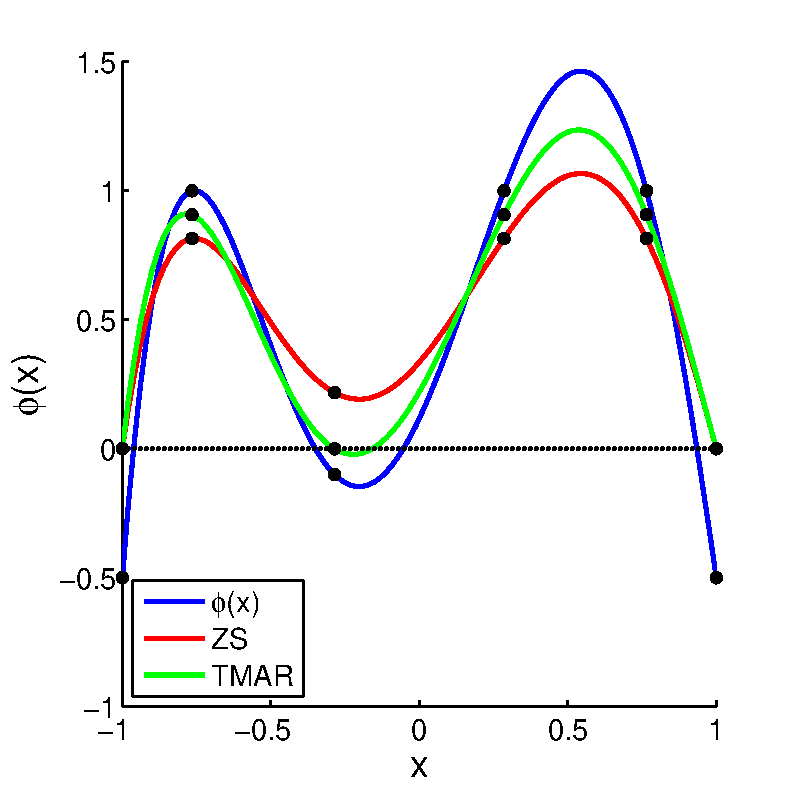
\includegraphics[width=0.5\textwidth]{figs/1d/zsTMAR_compareEx.pdf}
\caption{Fifth degree polynomial $\phi(x)$ with three negative GLL values (blue). Linear rescaling modification to $\phi(x)$ (red). TMAR modification to $\phi(x)$ (green). GLL points shown with black dots. } \label{fig:polyModCompare}
\end{figure}

Figure~\ref{fig:polyModCompare} illustrates the difference between the linear rescaling used in the ZS limiter (shown in red) and the TMAR adjustment described above (shown in green) when applied to a fifth degree polynomial $\phi(x)$ (shown in blue) which has negative values at three of the GLL nodes: two at the element edges and one near the center. After applying the linear rescaling, the two largest magnitude negative nodal values have been scaled zero while the smaller magnitude negative in the center is pushed into positive values. Moving this node into positive values requires that more mass be pulled away from the other positive nodes in order to maintain conservation. The result is a modified polynomial has been noticeably damped compared to the original polynomial. The impact of the TMAR modification on $\phi$ is less severe because the modification is nonlinear: all negative nodal values are set exactly to zero while non-negative values undergo a separate reduction. Rather than being pushed into positive values, the central negative is set to zero which requires that less mass be removed from the non-negative nodes to compensate.

Finally, we conclude this section by showing that the TMAR limiter does not alter the uniform high--order accuracy as the element spacing is refined.
\begin{thm} \label{thm:acc}
Let $\phi_{s_i}(x)$ be the unmodified $M$th order DG approximation to $\psi(x)$ in $s_i$ and assume that $\pbar{\phi}_{s_i} \geq 0$. Then the TMAR limited solution \eqref{eq:tmar} is also an $M$th order approximation to $\psi(x)$.
\end{thm}
\begin{pf}
Because $\phi_{s_i}(x)$ is an $M$th order approximation to $\psi(x)$
\al{
\max_{x\in s_i} \left| \psi(x) - \phi_{s_i}(x) \right| = \mathcal{O}(\dx^{M}).
}
it suffices to show that 
\al{
\max_{x\in s_i} \left| \phi^*_{s_i}(x) - \phi_{s_i}(x) \right| = \mathcal{O}(\dx^{M}).
}
Since the coefficients in the Legendre polynomial representation of $\phi^*_{s_i}(x)$ are given by the modified nodal values in \eqref{eq:tmar},
\al{
\max_{x\in s_i} \left| \phi^*_{s_i}(x) - \phi_{s_i}(x) \right| &= \max_{x\in s_i}  \left| \sum_{k=0}^N \left( \phi^*_{s_i}(x_k) - \phi_{s_i}(x_k) \right) \varphi_k(x) \right| \\
&\leq C_N \sum_{k=0}^N \left| \phi^*_{s_i}(x_k) - \phi_{s_i}(x_k) \right| 
}
where $C_N$ is a constant which depends only on $N$. Thus we need to show that $\sum_{k=0}^N \left| \phi^*_{s_i}(x_k) - \phi_{s_i}(x_k) \right| = \mathcal{O}(\dx^{M})$. 

There are two cases to consider. First suppose that $\phi_{s_i}(x_k) \leq 0$, then $\phi_{s_i}^*(x_k) = 0$, so $\phi_{s_i}(x_k) \leq \phi^*_{s_i}(x_k) \leq \psi(x_k)$. Since $\phi_{s_i}(x)$ is an approximation to $\psi$ with error $\mathcal{O}(\dx^{M})$, it follows that
\al{ \label{eq:thmBnd1}
\left| \phi^*_{s_i}(x_k) - \phi_{s_i}(x_k) \right| \leq \left| \psi(x_k) - \phi_{s_i}(x_k) \right| = \mathcal{O}(\dx^{M}).
}
On the other hand suppose that $\phi_{s_i}(x_k) > 0$, then $\phi_{s_i}^*(x_k) = r_i \phi_{s_i}(x_k)$ where $r$ is given in \eqref{eq:rdef}. Noting that $r_i \leq 1$,
\al{ \label{eq:thmBnd2}
\left| \phi^*_{s_i}(x_k) - \phi_{s_i}(x_k) \right| = (1-r_i)\phi_{s_i}(x_k).
}
Defining 
\al{
\phi_{s_i}^{+}(x_l) = 
	\begin{cases}
	\phi_{s_i}(x_l) & \mbox{if } \phi_{s_i}(x_l) \geq 0 \\
	0 & \mbox{if } \phi_{s_i}(x_l) < 0
	\end{cases} \mbox{ and} \quad
\phi_{s_i}^{-}(x_l) = 
	\begin{cases}
	0 & \mbox{if } \phi_{s_i}(x_l) \geq 0 \\
	\phi_{s_i}(x_l) & \mbox{if } \phi_{s_i}(x_l) < 0
	\end{cases},
}
the coefficient $(1-r_i)$ may be rewritten as
\al{ \label{eq:1-r}
1-r_i = \frac{\sum\limits_{l=0}^N w_l \left| \phi_{s_i}^-(x_l) \right| }{\sum\limits_{l=0}^N w_l \left| \phi_{s_i}^+(x_l) \right|}. 
}
Substituting \eqref{eq:1-r} into \eqref{eq:thmBnd2} and using the inequality $\sum\limits_{l=0}^N w_l \left| \phi_{s_i}^+(x_l) \right| \geq w_k \phi_{s_i}(x_k)$ to bound the denominator in \eqref{eq:1-r} from below gives
\al{
\left| \phi^*_{s_i}(x_k) - \phi_{s_i}(x_k) \right| \leq \frac{1}{w_k} \sum\limits_{l=0}^N w_l \left| \phi_{s_i}^-(x_l) \right|.
}
From \eqref{eq:thmBnd1} it follows that $|\phi_{s_i}^{-}(x_l)| = \mathcal{O}(\dx^{M})$ for all $l=0,\dots,N$. Thus
\al{
\left| \phi^*_{s_i}(x_k) - \phi_{s_i}(x_k) \right| \leq D_N \dx^{M} = \mathcal{O}(\dx^{M}),
}
where $D_N$ is a constant which depends only on $N$. Therefore $\left| \phi^*_{s_i}(x_k) - \phi_{s_i}(x_k) \right| = \mathcal{O}(\dx^{M})$ for all $k$, and  the TMAR limiter maintains $M$th order accuracy relative to $h$--refinement.
\end{pf}

\section{Positivity Preservation in 2D} \label{sec:pp2d}

The TMAR limiter described in Section \ref{sec:pp1d} can be extended to two-dimensional (and higher) problems. Following the approaches of\cite{nair2005discontinuous} and \cite{Lauritzen:2011aa} we expand $\phi_{s_i}(x,y,t)$ by taking the tensor-product of the one-dimensional basis polynomials:
\al{
\phi_{s_i}(x,y,t) = \sum \limits_{k,l=0}^N a_{i,k,l}(t) \varphi_k (x) \varphi_l(y).
}
Let $\pbar{\phi}_{ij}$ denote the average value of the degree $N$ local discontinuous Galerkin (DG) approximating polynomial within element $S_{ij}$. A DG scheme for updating $\pbar{\phi}_{ij}$ in a forward Euler step can be written as
\al{ \label{2dFwd_1}
\pbar{\phi}_{ij}^{n+1} =  \pbar{\phi}_{ij}^{n} - \frac{\dt}{\dx \dy} \left[ \int_{y_{j-\haf}}^{y_{j+\haf}} \left( F_{i+\haf}(y) - F_{i-\haf}(y) \right) dy + \int_{x_{i-\haf}}^{x_{i+\haf}} \left( G_{j+\haf}(x) - G_{j-\haf}(x) \right) dx\right]
}
where $\dx$ and $\dy$ are the horizontal and vertical element sizes respectively, and $F_{i\pm\haf}(y)$ and $G_{j\pm\haf}(x)$ are the horizontal and vertical numerical flux functions through the east/west and north/south interfaces. Equation \eqref{2dFwd_1} can be rewritten more compactly in terms of the mean fluxes $\pbar{F}_{i\pm \haf}$ and $\pbar{G}_{j\pm \haf}$ through each interface as 
\al{\label{2dFwd_avg}
\pbar{\phi}_{ij}^{n+1} =  \pbar{\phi}_{ij}^{n} - \frac{\dt}{\dx \dy} \left[ \dy \left( \pbar{F}_{i+\haf} - \pbar{F}_{i-\haf}\right) + \dx \left( \pbar{G}_{j+\haf} - \pbar{G}_{j-\haf} \right) \right].
}
Notice that equation \eqref{2dFwd_avg} is in the same form as a finite volume update to $\pbar{\phi}_{ij}^{\,n}$ which uses the mean fluxes. With this in mind, we apply the standard multidimensional FCT algorithm presented by Zalesak in \cite{Zalesak:1979aa} to \eqref{2dFwd_avg} in order to determine the corrected mean fluxes $\pbar{F}_{i\pm\haf}^{\,*}$ and $\pbar{G}_{j\pm\haf}^{\,*}$ which will not drive $\pbar{\phi}_{ij}^{\,n}$ negative. For completeness, this approach is summarized below:
\begin{enumerate}
\item Let $Q_{ij}$ be the maximum outward flux sustainable over a single time step without forcing $\pbar{\phi}_{ij}^{n+1}$ negative,
\al{
Q_{ij} = \frac{\pbar{\phi}_{ij}^{\,n} \dx \dy}{\dt}. \nono
}
\item Let $P_{ij}$ be the the net mean flux out of the element, given by
\al{
P_{ij} = \dy \left[ \max \left( 0,\pbar{F}_{i+\haf} \right) - \min \left( 0,\pbar{F}_{i-\haf}  \right) \right] + \dx \left[ \max \left( 0,\pbar{G}_{j+\haf} \right) - \min \left( 0,\pbar{G}_{j-\haf}  \right) \right]. \nono 
}
\item Next, determine the ratio by which the mean fluxes need to be corrected to ensure that a negative will not generated,
\al{
R_{ij} = \min \left( 1, \frac{Q_{ij}}{P_{ij} + \epsilon }\right) \nono
}
where $\epsilon$ is a small parameter (like $10^{-10}$) which is added to avoid division by zero.
\item Finally, the corrected mean fluxes are given using the correction ratio from whichever element the fluxes are actually removing material from
\al{
\pbar{F}_{i+\haf}^{\,*} = 
	\begin{cases} 
	R_{ij} \pbar{F}_{i+\haf} & \mbox{\rm if } \pbar{F}_{i+\haf} \geq 0 \\
	R_{i+1j} \pbar{F}_{i+\haf} & \mbox{\rm if } \pbar{F}_{i+\haf}< 0 \end{cases}.  \nono
}
\end{enumerate}

This approach yields a modification to the mean fluxes which will keep $\pbar{\phi}_{ij}$ nonnegative. However, in practice it is the pointwise fluxes which have been evaluated at quadrature locations around the boundary of the element that appear in the simulated  DG equations, rather than the mean fluxes. Therefore it is necessary to translate the modification to the mean fluxes into an equivalent modification of the pointwise fluxes. The integrals in \eqref{2dFwd_1} are approximated using quadrature rules of sufficient accuracy. Suppose that the interval $[x_{i-\haf} , x_{i+\haf}]$ has been mapped to the reference interval $[-1,1]$ and let $\xi_k$ and $w_k$ $k=0,\dots,N$ denote the one-dimensional GLL quadrature points and weights for this interval. The mean flux through the $i+\haf$ interface is given in terms of the pointwise fluxes $F_{i+\haf}(\xi_k)$ by
\al{ \label{meanFlxAppx}
\pbar{F}_{i+\haf} = \frac{1}{2}\sum\limits_{k=0}^N w_k F_{i+\haf}(\xi_k).
}
In particular, equation \eqref{meanFlxAppx} expands $\pbar{F}_{i+\haf}$ in a linear combination of the pointwise fluxes. The simplest approach for translating the FCT technique above into a modification to the point fluxes is to linearly apply the correction factor for the mean flux to each pointwise flux. In other words, if $\pbar{F}_{i+\haf}^{\,*} = c \pbar{F}_{i+\haf}$ for some correction factor $0\leq c \leq1$ then the modified nodal fluxes $F_{i+\haf}^{\,*}(\xi_k)$ which will be used in the forward step are given by
\al{
F_{i+\haf}^{\,*}(\xi_k) = c F_{i+\haf}(\xi_k).
}

Once the element mean is non-negative, adapting the TMAR limiter to 2d is relatively simple and requires updating the quadrature weights in\eqref{eq:rdef} to take into account the new tensor product quadrature rule and summing over all nodes:
\al{
r_{i} = \frac{\pbar{\phi}_{s_i}}{\sum \limits_{k,l=0}^N w_k w_l ( \phi_{s_i}(x_k,y_l) + | \phi_{s_i}(x_k,y_l) |  )/2}.
}
The limited nodal values for $k,l=0,\dots,N$ are given by
\al{
\phi^*_{s_i}(x_k,y_l) = 
        \begin{cases} 
         0 & \mbox{if } \phi_{s_i}(x_k,y_l) < 0 \\
        r_i \phi_{s_i}(x_k,y_l) & \mbox{if } \phi_{s_i}(x_k,y_l) > 0 
        \end{cases}.
}
A similar proof to the one described in Theorem \ref{thm:acc} also shows that this 2d limiting method does not reduce the asymptotic convergence rate of the underlying DG approximation.

\section{Numerical Tests} \label{sec:numTest}
\subsection*{One-dimensional tests}
Each of the one-dimensional tests we study use constant windspeed $u=1$ on a periodic domain $\Omega = [0,1]$. The exact solution for all $x$ and $t$ is given by the translation $\psi(x,t) = \psi_0(x-t)$. We will consider several several sets of initial conditions, all of which satisfy the non-negativity condition. For the unlimited and TMAR methods, the time step taken is determined based on the maximum possible Courant--Friedrichs--Lewy (CFL) number $\mu = \frac{\max |u| \dt}{\dx}$ for stability. For methods implementing the ZS limiter a second time step condition is given in \cite{Zhang2010} which is necessary to guarantee non-negativity. If $L$ is the smallest integer for which an $L$-point GLL quadrature for the interval $[-1,1]$ with weights $\hat{w}_k$ is exact for polynomials of degree $N$, then the appropriate CFL condition is 
\al{\label{zsCFL}
\mu \leq \min_{k} \frac{\hat{w}_k}{2}.
}
Table \ref{cflTable} lists numerical values for the maximum permissible CFLs for several polynomial degrees using SSPRK3 time stepping. In all of the following one-dimensional tests we use a time step given by $\mu = 0.8 \mu_{\text{max}}$. 

\begin{table}[!hb]
\begin{tabular}{cccc}
\toprule
& \multicolumn{3}{c}{$\mu_{\text{max}}$} \\ \cline{2-4} 
Degree  & Modal & Nodal & ZS \\
\midrule
2 & 0.210 & 0.450 & 0.167 \\
3 & 0.130 & 0.255 & 0.167 \\
4 & 0.090 & 0.168 & 0.083 \\
5 & 0.067 & 0.120 & 0.083 \\
\bottomrule
\end{tabular}
\caption{Maximum permissible 1D CFL values for DG methods of polynomial degree 2 through 5 schemes with SSPRK3 time stepping. ZS values are from \cite{Zhang2010}; Modal and nodal values from \cite{ullrichWaves2013} (without normalization).}
\label{cflTable}
\end{table}

We first consider the advection of a square profile
\al{
 \psi_0(x) =\begin{cases} 1 & \mbox{\rm if } x\in [0.4,0.6] \\
               		            0 & \mbox{otherwise} \end{cases}.
}
Figure \ref{fig:sqwave} displays the unlimited, TMAR, and ZS limited numerical solutions at time $t=5$ (after five cycles around the periodic domain) using piecewise quartic polynomials and sixteen elements. Each dot in Fig.~\ref{fig:sqwave} indicates the polynomial value at one of the 5 GLL nodes. The $L_2$ and $L_{\infty}$ norms, along with the maximum and minimum values are also listed in each panel. The spurious negatives present in the unlimited solution (Fig.~\ref{fig:sqwave}a) are completely removed by both limiting methods (Fig.~\ref{fig:sqwave}b and c) with only a slight increase in each of the error norms. Both limiters produce roughly equivalent $L_2$ and $L_{\infty}$ errors and similar visual improvements compared to the unlimited solution. The only noticeable difference between the limited solutions is on the upwind side of the square wave where a small overshoot is more pronounced in the ZS solution.

\begin{figure}
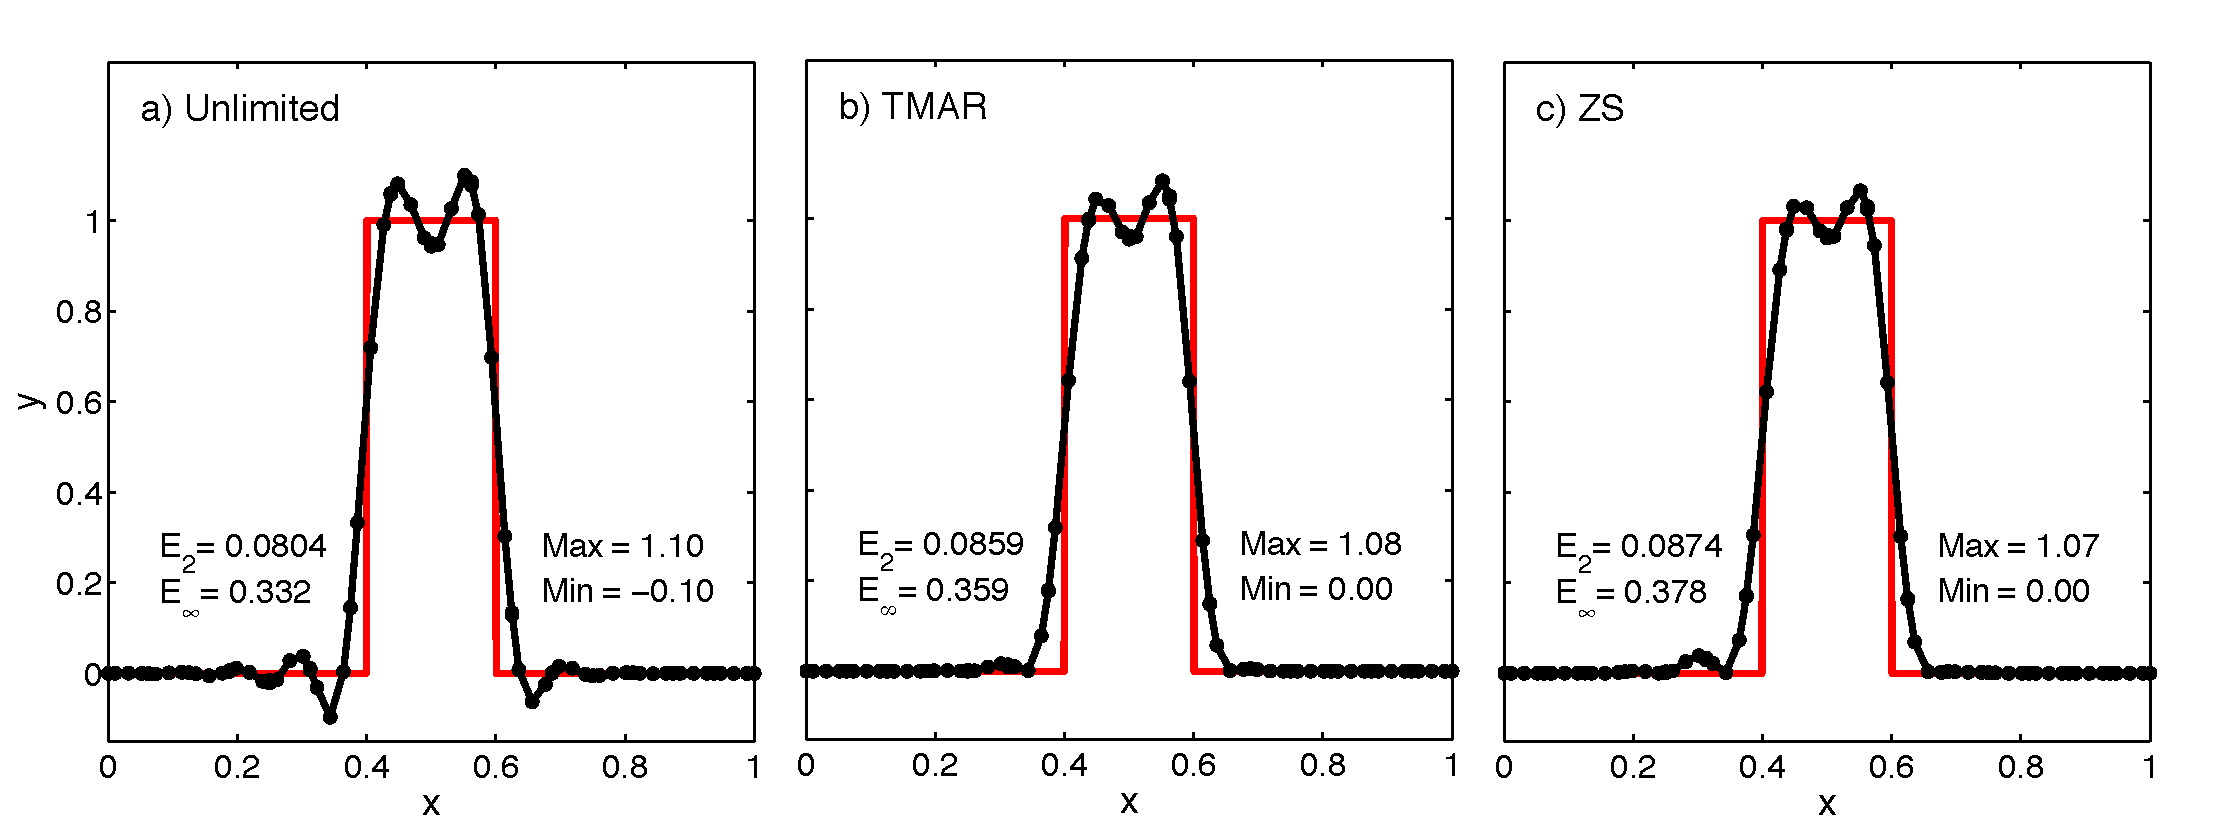
\includegraphics[width=\textwidth]{figs/1d/sqwaveCmpre_N4E16_nodal.pdf}
\caption{Constant speed advection of a square profile five times through a periodic domain using 16 elements and 4th degree polynomials: {\bf a)} Unlimited, {\bf b)} truncated and mass-aware, and {\bf c)} Zhang and Shu solutions.} \label{fig:sqwave}
\end{figure}

\begin{figure}
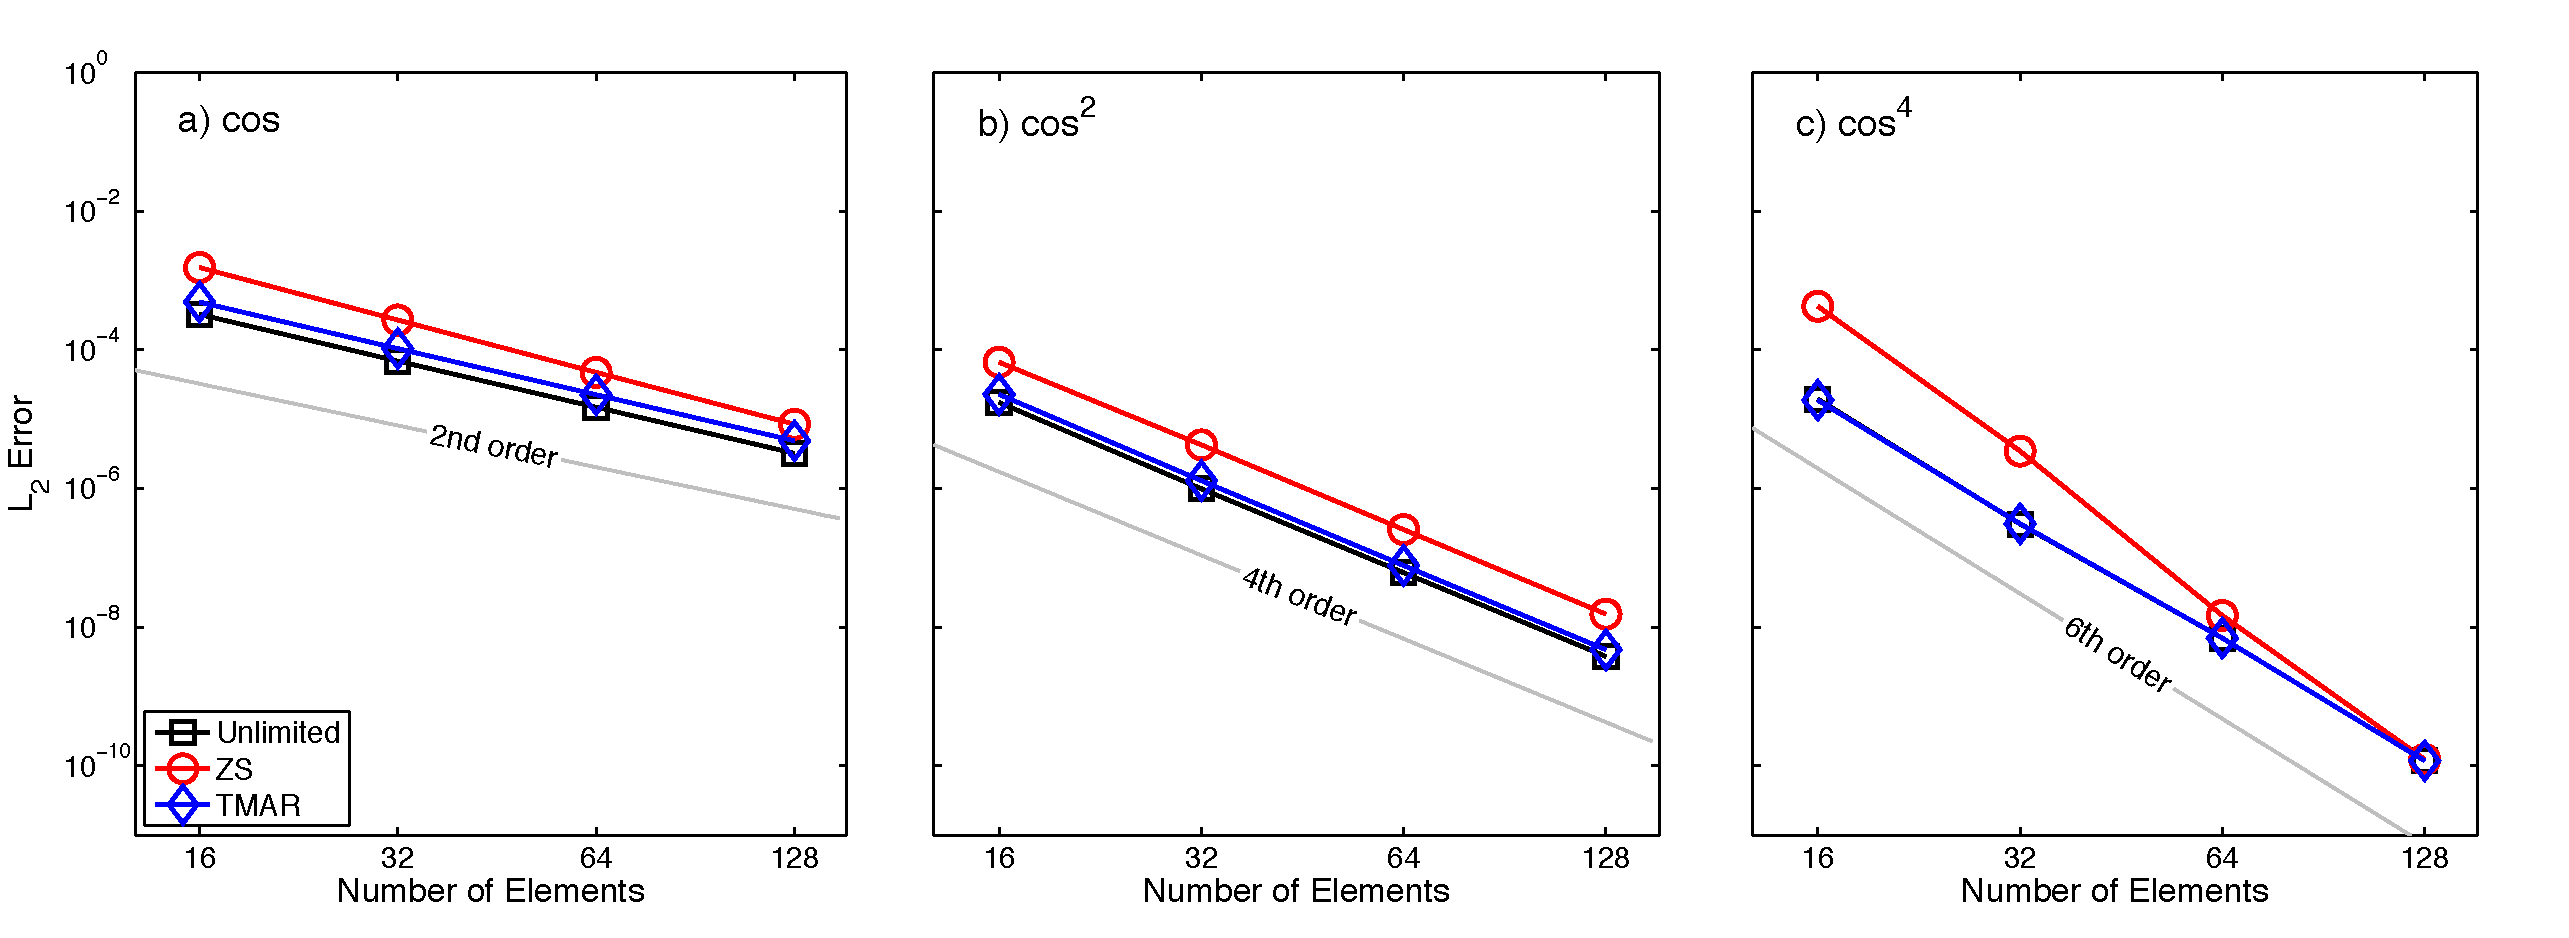
\includegraphics[width=\textwidth]{figs/1d/cosbell_hConvg_nodal.pdf}
\caption{Convergence results under $h$--refinement: $L_2$ error as a function of the number of elements for {\bf a)} $C^1$, {\bf b)} $C^3$ and, {\bf c)} $C^7$ cosine bell tests as defined by the initial conditions \eqref{eq:cosbell}. } \label{fig:cosConv-h}
\end{figure}

One of the most important benefits of implementing DG methods is that they they allow the flexibility of refining the approximate solution by either adding additional elements ($h$-refinement), using a higher degree local polynomials ($p$-refinement), or a combination of the two. Therefore, consider the influence of each limiter on the $h$- and $p$-convergence rates for smooth initial data. Let $s(x) = 4 \, |x-1/4|$ and define a  initial tracer density by the cosine bells
\al{ \label{eq:cosbell}
\psi_0(x) = \begin{cases}
       \displaystyle{\left( \frac{1+\cos(\pi s(x) )}{2} \right)^{p}} & \mbox{\rm if } s(x) \le 1 \\
       0 & \mbox{\rm otherwise} \end{cases},
}
where  $p=1,2,$ or $4$.  By design $\psi_0(x)$ in \eqref{eq:cosbell} is $C^{2p-1}$ so larger $p$ values permit faster convergence rates depending on the degree of the DG polynomial truncation. No matter what value of $p$ is used, the initial profile features steep gradients so that the unlimited solution will develop small negative densities. Figure~\ref{fig:cosConv-h} illustrates the impact of each limiting method on $h$-convergence in the $L_2$ error. All three methods use fifth degree polynomials with a time step chosen for SSPRK3 integration so that $\dt \sim \mathcal{O} ( \dx^{5/3} )$ to guarantee that spatial convergence is observed. As expected, the effective order of accuracy (i.e. the slope) of the limited solutions closely match that of the unmodified method. Note, however, that for all three initial conditions the error generated by the TMAR limiter is smaller in magnitude than that produced by the ZS limiter. 

Figure~\ref{fig:cosConv-p} examines the $p$--convergence for the same set of initial conditions as $N$ is refined from 4 to 9. Each method uses a fixed mesh of $32$ elements and a time step $\dt = \dx^{N/3}/2$ which ensures that spatial convergence is observed. The unlimited solution generates the fastest convergence rate for the smoothest cosine bell which begins to slow as errors begin to approach machine precision for the highest degree truncations. This is expected since as the smoothness of the solution increases, $p$--refinement should begin to produce spectrally convergent results. The TMAR limited solution introduces slightly larger errors than the unlimited scheme, but nevertheless parallels the unlimited solution's convergence for all three initial conditions. On the other hand, $p$--refinement produces little to no improvement in the ZS limited solution for the $C^1$ and $C^3$ cosine bells and only modest improvement for the smoothest example. Therefore, while both limiters maintain the original method's convergence rate under $h$--refinement, we find that only the TMAR limiter maintains the performance under $p$--refinement for a fixed spatial grid. This difference under $p$--refinement is further investigated in the two-dimensional tests.

\begin{figure}
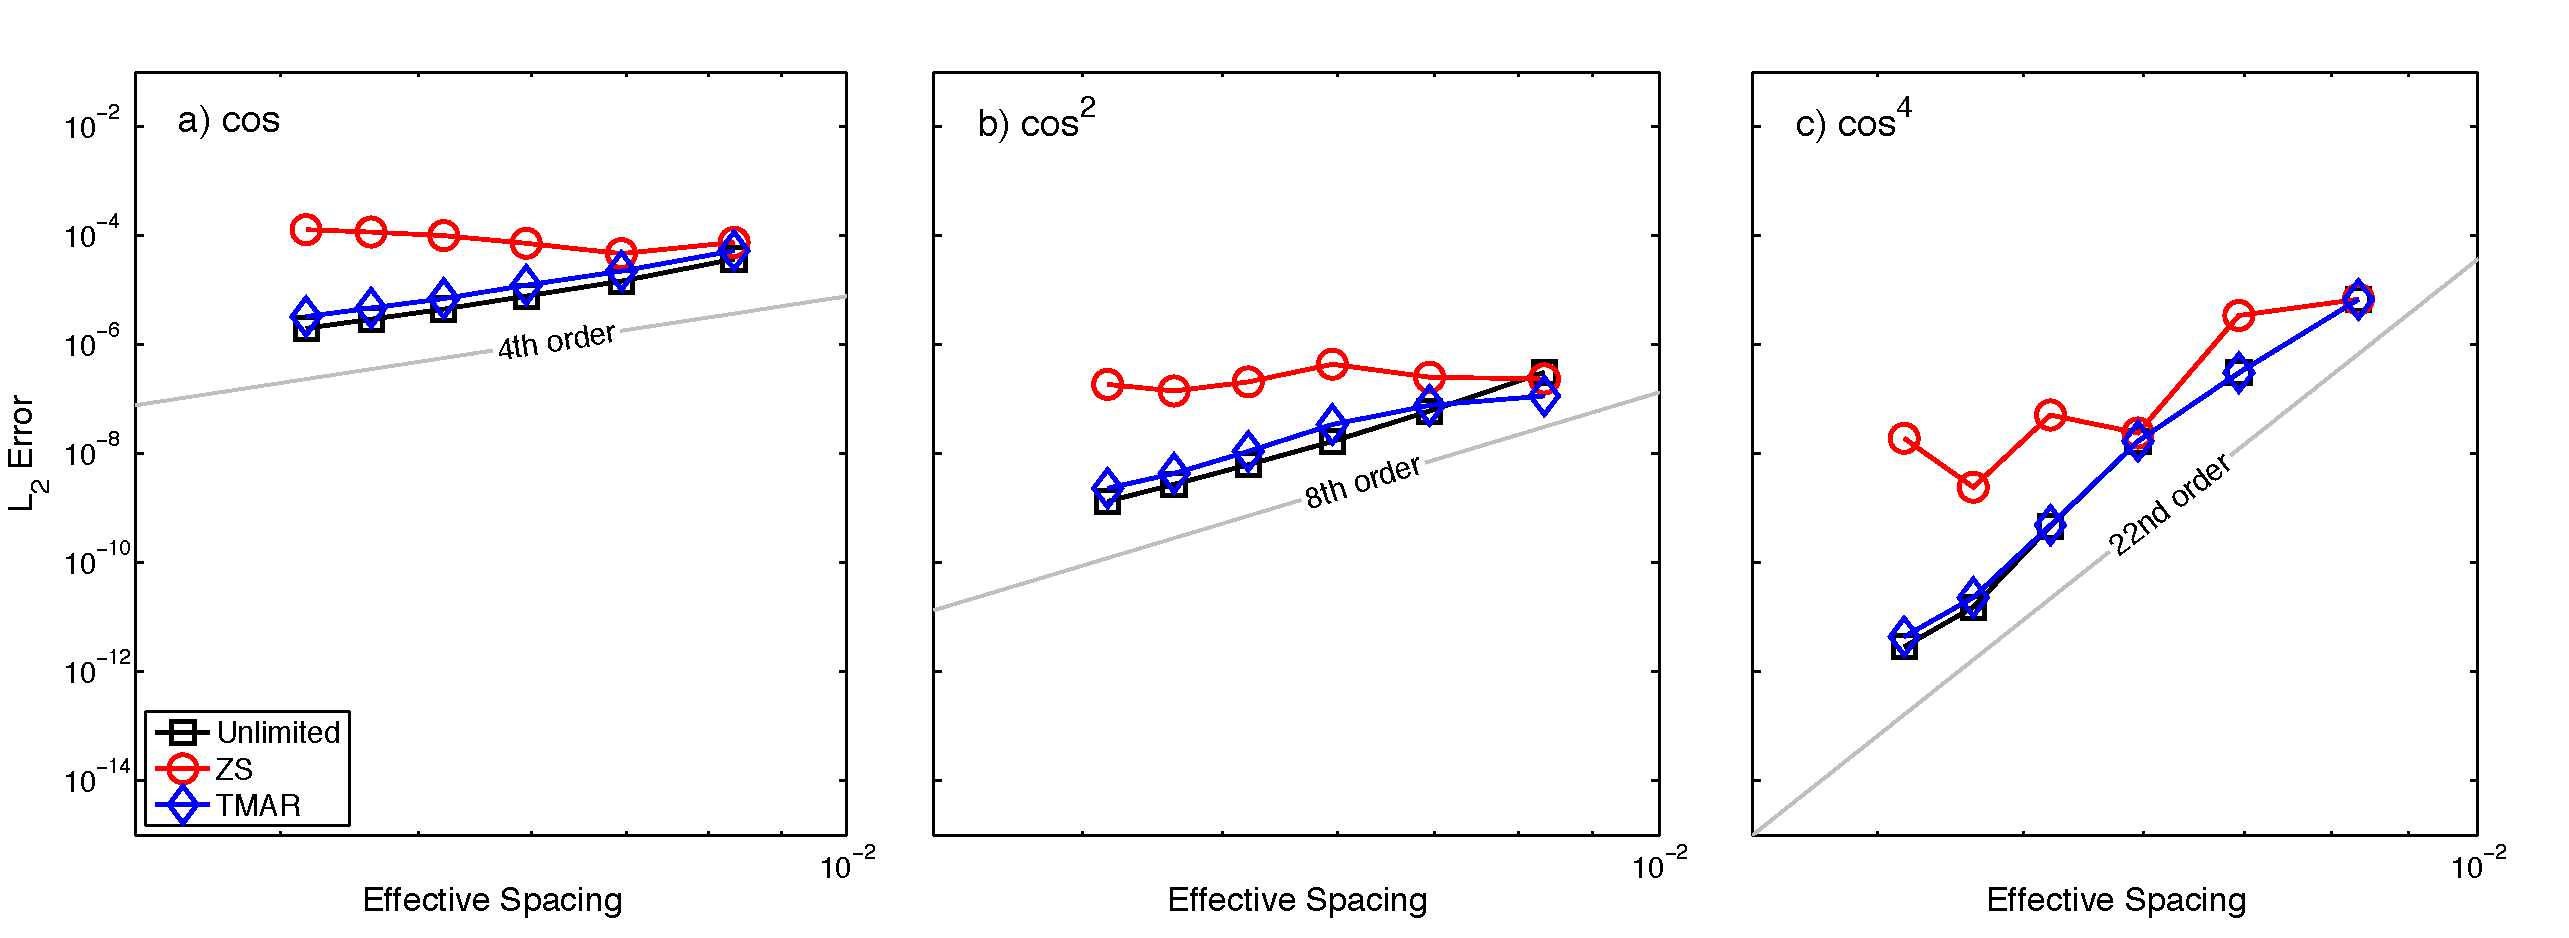
\includegraphics[width=\textwidth]{figs/1d/cosbellConvg_nodal.pdf}
\caption{Convergence results under $p$--refinement: $L_2$ error for {\bf a)} $C^1$, {\bf b)} $C^3$ and, {\bf c)} $C^7$ cosine bell tests. Each test uses a 32 element mesh.} \label{fig:cosConv-p}
\end{figure}

\subsection*{Two-dimensional tests}

In multi-dimensional problems, complex velocity fields can stretch and deform smooth initial data into filaments with poorly resolved steep gradients regardless of how well the initial conditions are resolved.  This behavior can be replicated by using a time-dependent velocity field to deform an initially circular tracer distribution into a narrow coil before reversing and returning the tracer to its original shape. We will use the unit square domain  $\Omega = [0,1] \times [0,1]$. The non-divergent velocity field originally proposed in \cite{LeVeque1996} is defined over a time interval $0 \leq t \leq T=5$ by the streamfunction
\al{
{\Psi}(x,y,t) = \frac{1}{\pi} \sin(\pi x)^2  \sin ( \pi y )^2 \cos \left( \frac{\pi t}{T} \right), 
}
and the relations
\al{ \label{eq:2dDefVel}
 u = \frac{\partial {\Psi}}{\partial y}, \quad
 v = -\frac{\partial {\Psi}}{\partial x}.
}
The initial condition $\psi_0(x,y)$ is specified by \eqref{eq:cosbell} with $p=2$ and $s(x)$ replaced by the two--dimensional extension
\al{
s(x,y)  = 4 \left ( \left (x-\frac{1}{4}\right )^2 + \left (y-\frac{1}{4}\right )^2 \right )^{1/2}.
\label{2d_radius}
}
Tests using this same flow and the $C^3$ initial condition were also considered in \cite{ullrich2014}. Figure~\ref{fig:cosbellExact}a shows contours for the exact solution at $t=0$ and $T$, while Fig.~\ref{fig:cosbellExact}b shows a reference solution obtained using very high time and space resolution at the time of maximum deformation $t=T/2$. This test is significantly more challenging to limit because the relatively well resolved initial conditions are deformed into a very steep thin filament before the flow reverses. 

\begin{figure}
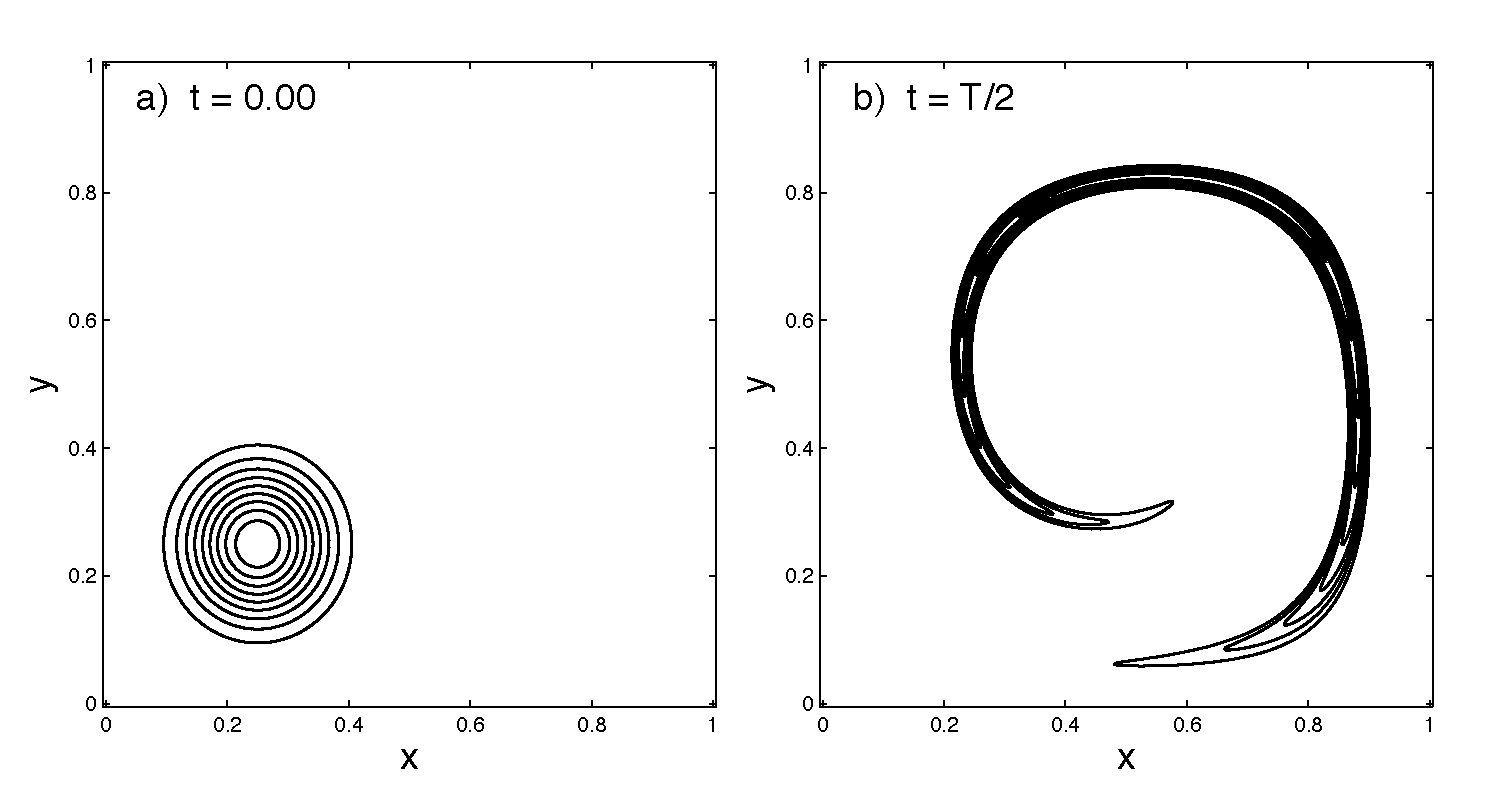
\includegraphics[width=0.8 \textwidth]{figs/2d/defCosbellExact.pdf}
\caption{Tracer concentration field for the $C^3$ cosine bell in the reversing deformation flow \eqref{eq:2dDefVel} at times \textbf{a)} 0 and $T$, and  \textbf{b)} $T/2$. Contours at intervals of 0.1.}
\label{fig:cosbellExact}
\end{figure}

For our two dimensional tests we will examine results of the proposed limiter when applied to both a fully two-dimensional DG method as well as DG methods which use dimensional splitting (originally proposed by Strang in \cite{strang68}) to update the two-dimensional solution in a series of one-dimensional updates. Since they involve a sequence of one-dimensional updates, the maximum time step for the Strang split methods remains the same as those allowed for each individual step listed in Table~\ref{cflTable}. A fully multidimensional DG method has a maximum stable $\Delta t$ which is reduced by a factor of $\sqrt{2}$ from the values listed in Table \ref{cflTable}. Turning to the positive-definite methods, there is no further reduction in maximum time step required by the TMAR limiter. The dimensional split ZS scheme must still satisfy \eqref{zsCFL} whereas the fully multidimensional ZS scheme must follow the more restrictive time step condition as derived in \cite{Zhang2010}: 
\begin{equation}
\mu_x + \mu_y \leq \min \limits_{k} \frac{w_k}{2}
\label{eqn:2dZScfl}
\end{equation}
where 
\al{
\mu_x = \max \limits_{(x,y) \in \Omega}|u| \frac{\Delta t}{\Delta x}, \quad \mu_y = \max \limits_{(x,y) \in \Omega}|v|  \frac{\Delta t}{\Delta y}. \nono
}
If the mesh is isotropic and $\max |u| = \max |v|$, this condition corresponds to a time step which is half as large as in the corresponding one-dimensional problem. Adopting a strategy similar to that in many practical applications, solutions we present obtained using a time step that brings the maximum local Courant number throughout the integration to no greater than 95\% of its limiting value.

Figure~\ref{fig:2dCosbell24} shows the results of each method for the deformation flow for a total of nine different limiter and method combinations. Each panel uses a $24 \times 24$ element grid with $N=4$ for a total of 120 degrees of freedom (DOFs) along each coordinate. Panels a), b), and c) use a fully two-dimensional nodal DG method, while panels the last two rows use dimensional splitting with nodal and modal basis functions respectively. Maximum and minimum values are listed in each panel, as well as the error measured from the analytic solution in $L^2$ and $L^{\infty}$ grid norms (listed as $E_2$ and $E_{\infty}$, respectively).

\begin{figure} 
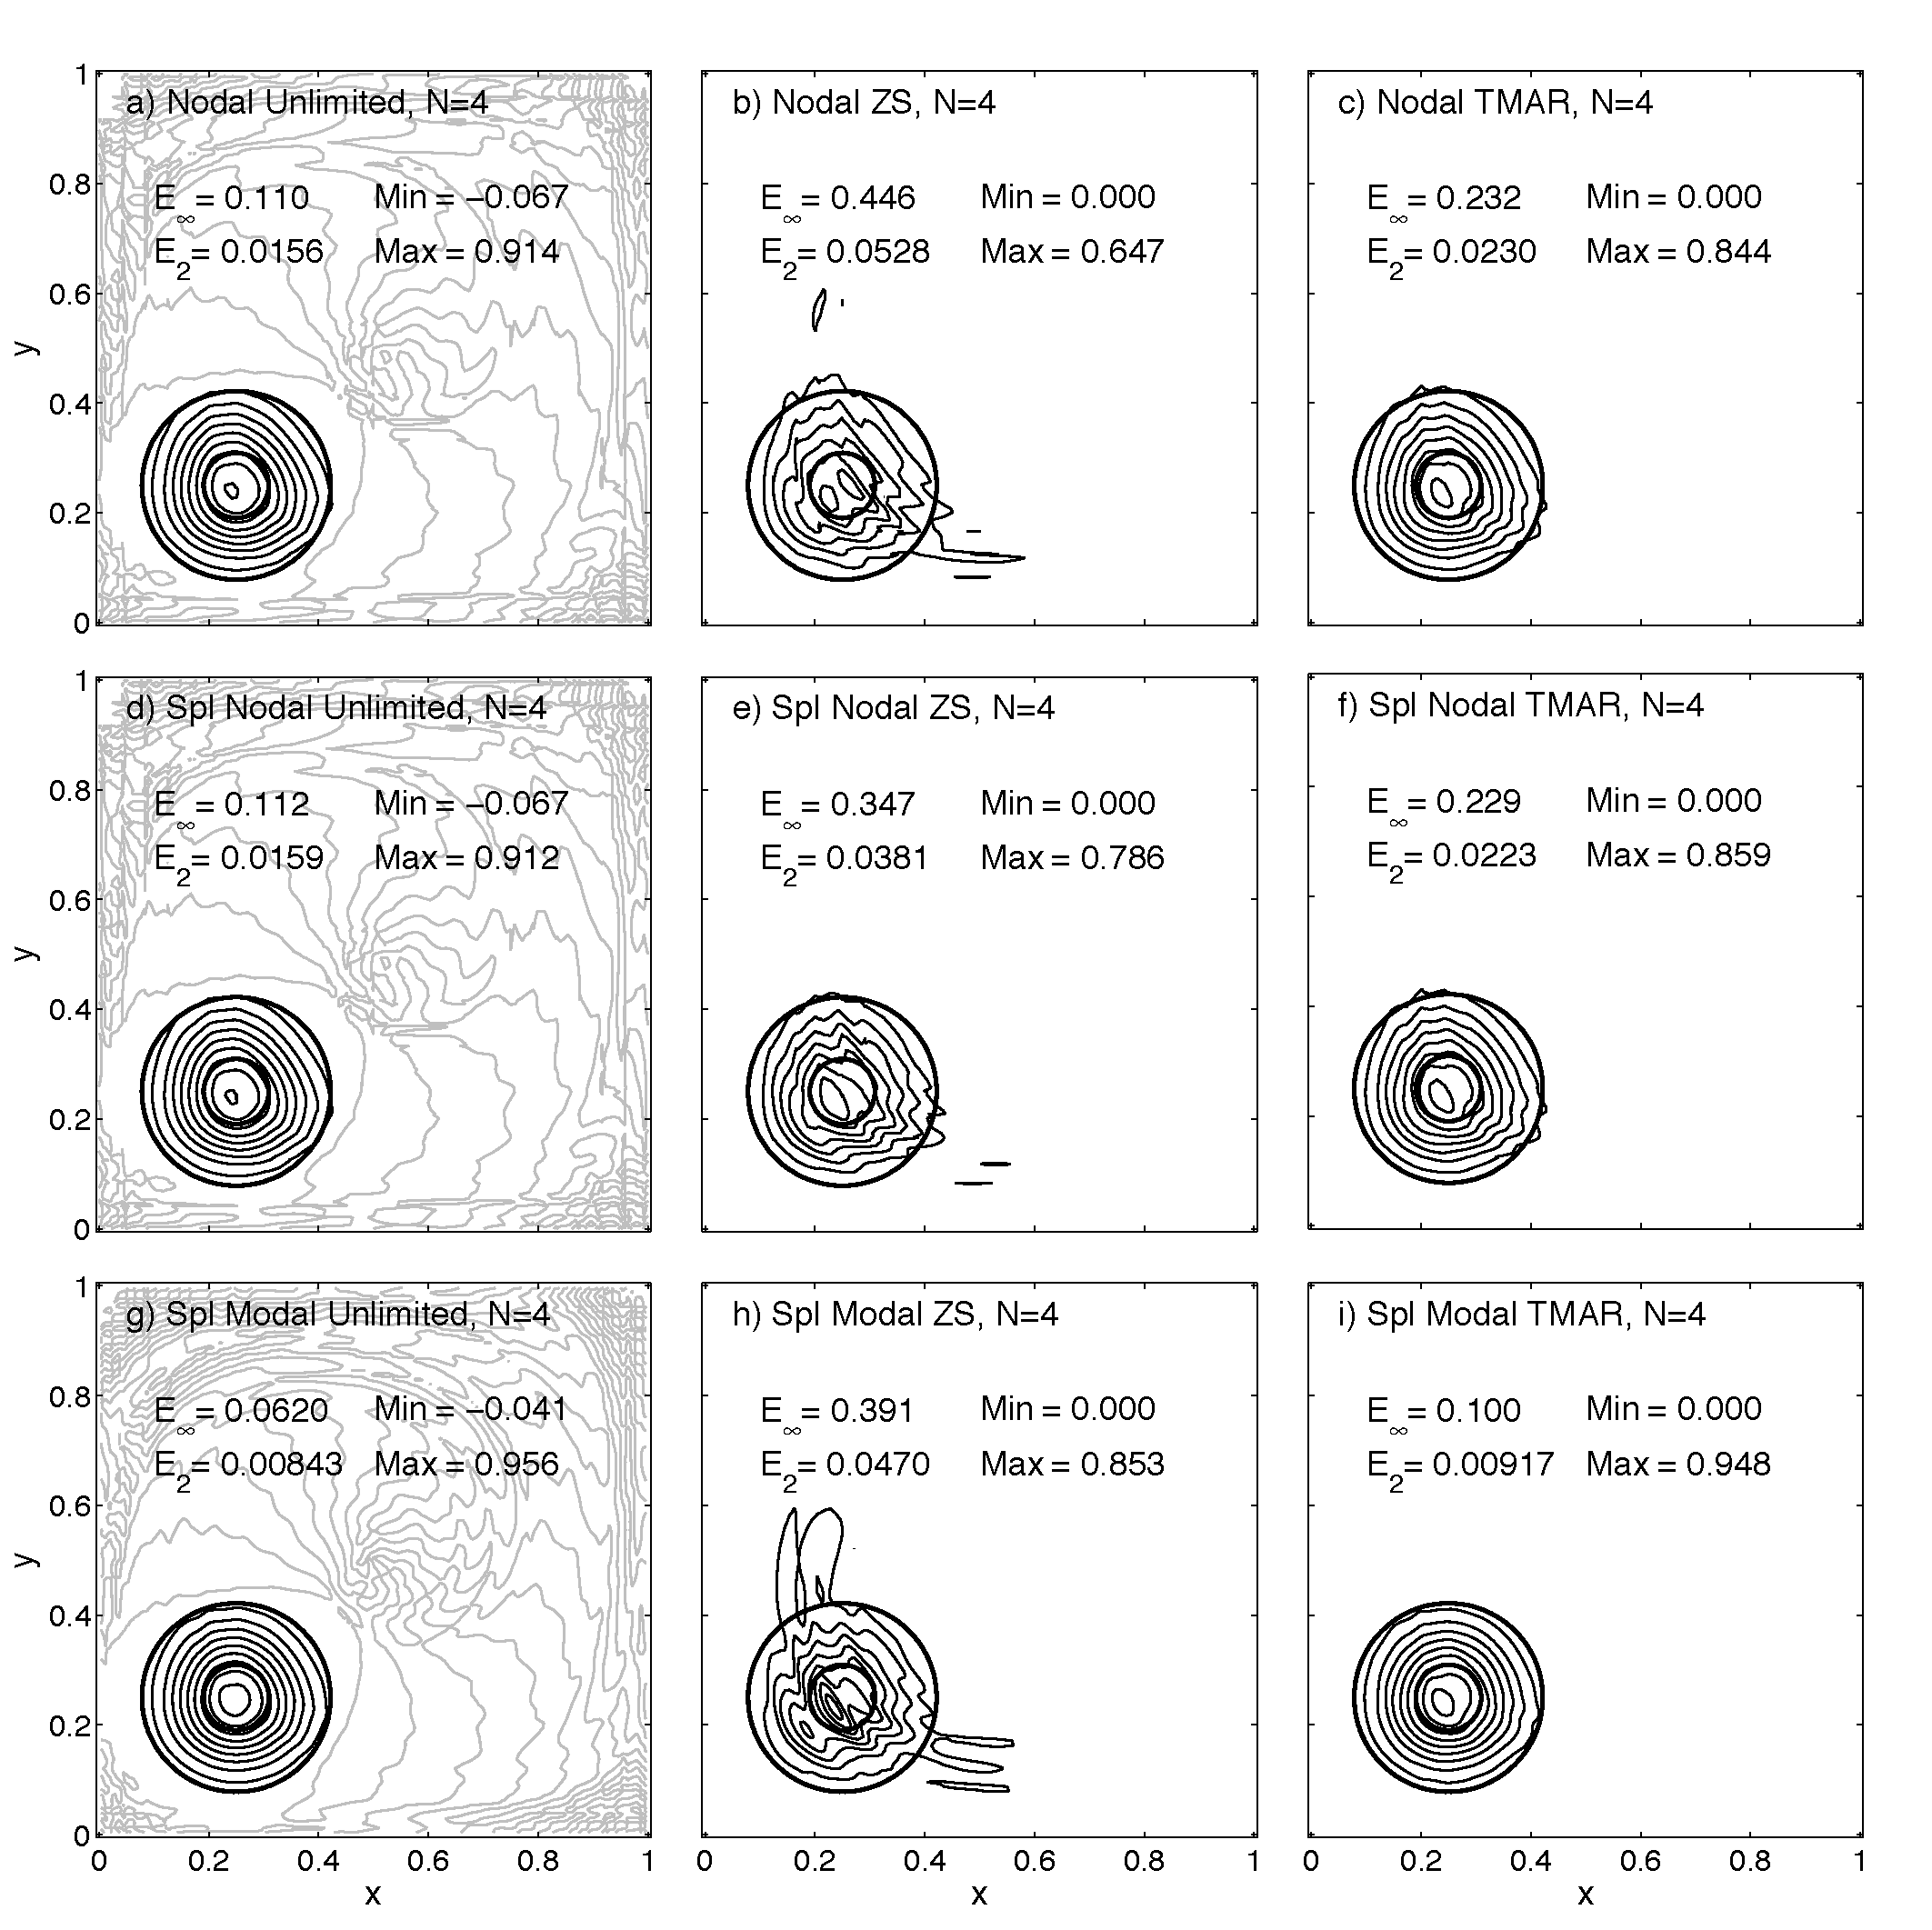
\includegraphics[width=\textwidth]{figs/2d/_defCosbell_9pan_24e.pdf}
\caption{Comparison of tracer concentration fields at $t=T$. Each panel uses the same $24\times24$ element grid. The limiting scheme and degree at which the polynomial expansions are truncated are given in each panel. Contours are every 0.1 and negative contours are highlighted in light gray. Exact solution contours at 0.05 and 0.75 shown in heavy solid lines}\label{fig:2dCosbell24}
\end{figure}

Each of the unlimited approximations does a fair job of maintaining the original amplitude of the exact solution after deformation as well as correctly estimating the the location of the peak. The presence of Strang splitting appears to have little impact on the quality of the solution, indicating that spatial errors are dominant at this resolution. However, as expected all three unlimited methods permit spurious negatives, shown with light gray contours, of magnitude between 4 and 7 percent of the initial amplitude of the bell. These negatives are completely removed in all of the limited solutions. Except for the elimination of all negative tracer densities, the TMAR limited solutions look similar in quality to their unlimited counterparts. The TMAR limited nodal solutions do see a 5-7\% decrease in their global maximum and a noticeable increase in both error norms, however the TMAR limited modal result sees a less than 1\% decrease in maximum amplitude and almost no change in $E_2$. Finally, notice that the TMAR limited modal solution exhibits better errors than both of the {\it unlimited} nodal solutions. In contrast, all of the ZS limited solutions have noticeably degraded the original solution, with substantial distortion of the tracer field, including segmentation of part of the solution away from the primary peak, a 12-25\% reduction in the global maximum, and a significant increase in both error norms. Results after doubling the number of elements along each coordinate to 48 are shown in Figure~\ref{fig:2dCosbell48}. At this resolution, the TMAR solutions look virtually identical to the unlimited solutions with the negatives removed and suffer very little degradation in the maximum amplitude. However, the relative performance of the TMAR solutions remains unchanged, with the modal solution remaining the best. The ZS limited solutions are also significantly improved compared to the Figure~\ref{fig:2dCosbell24} results. Most notably, there is no segmentation of the solution away from the peak. However there are still oscillations in the solution which are most visible in the outermost plotted contours and deviate from the circular symmetry present in the unlimited approximations.

\begin{figure} 
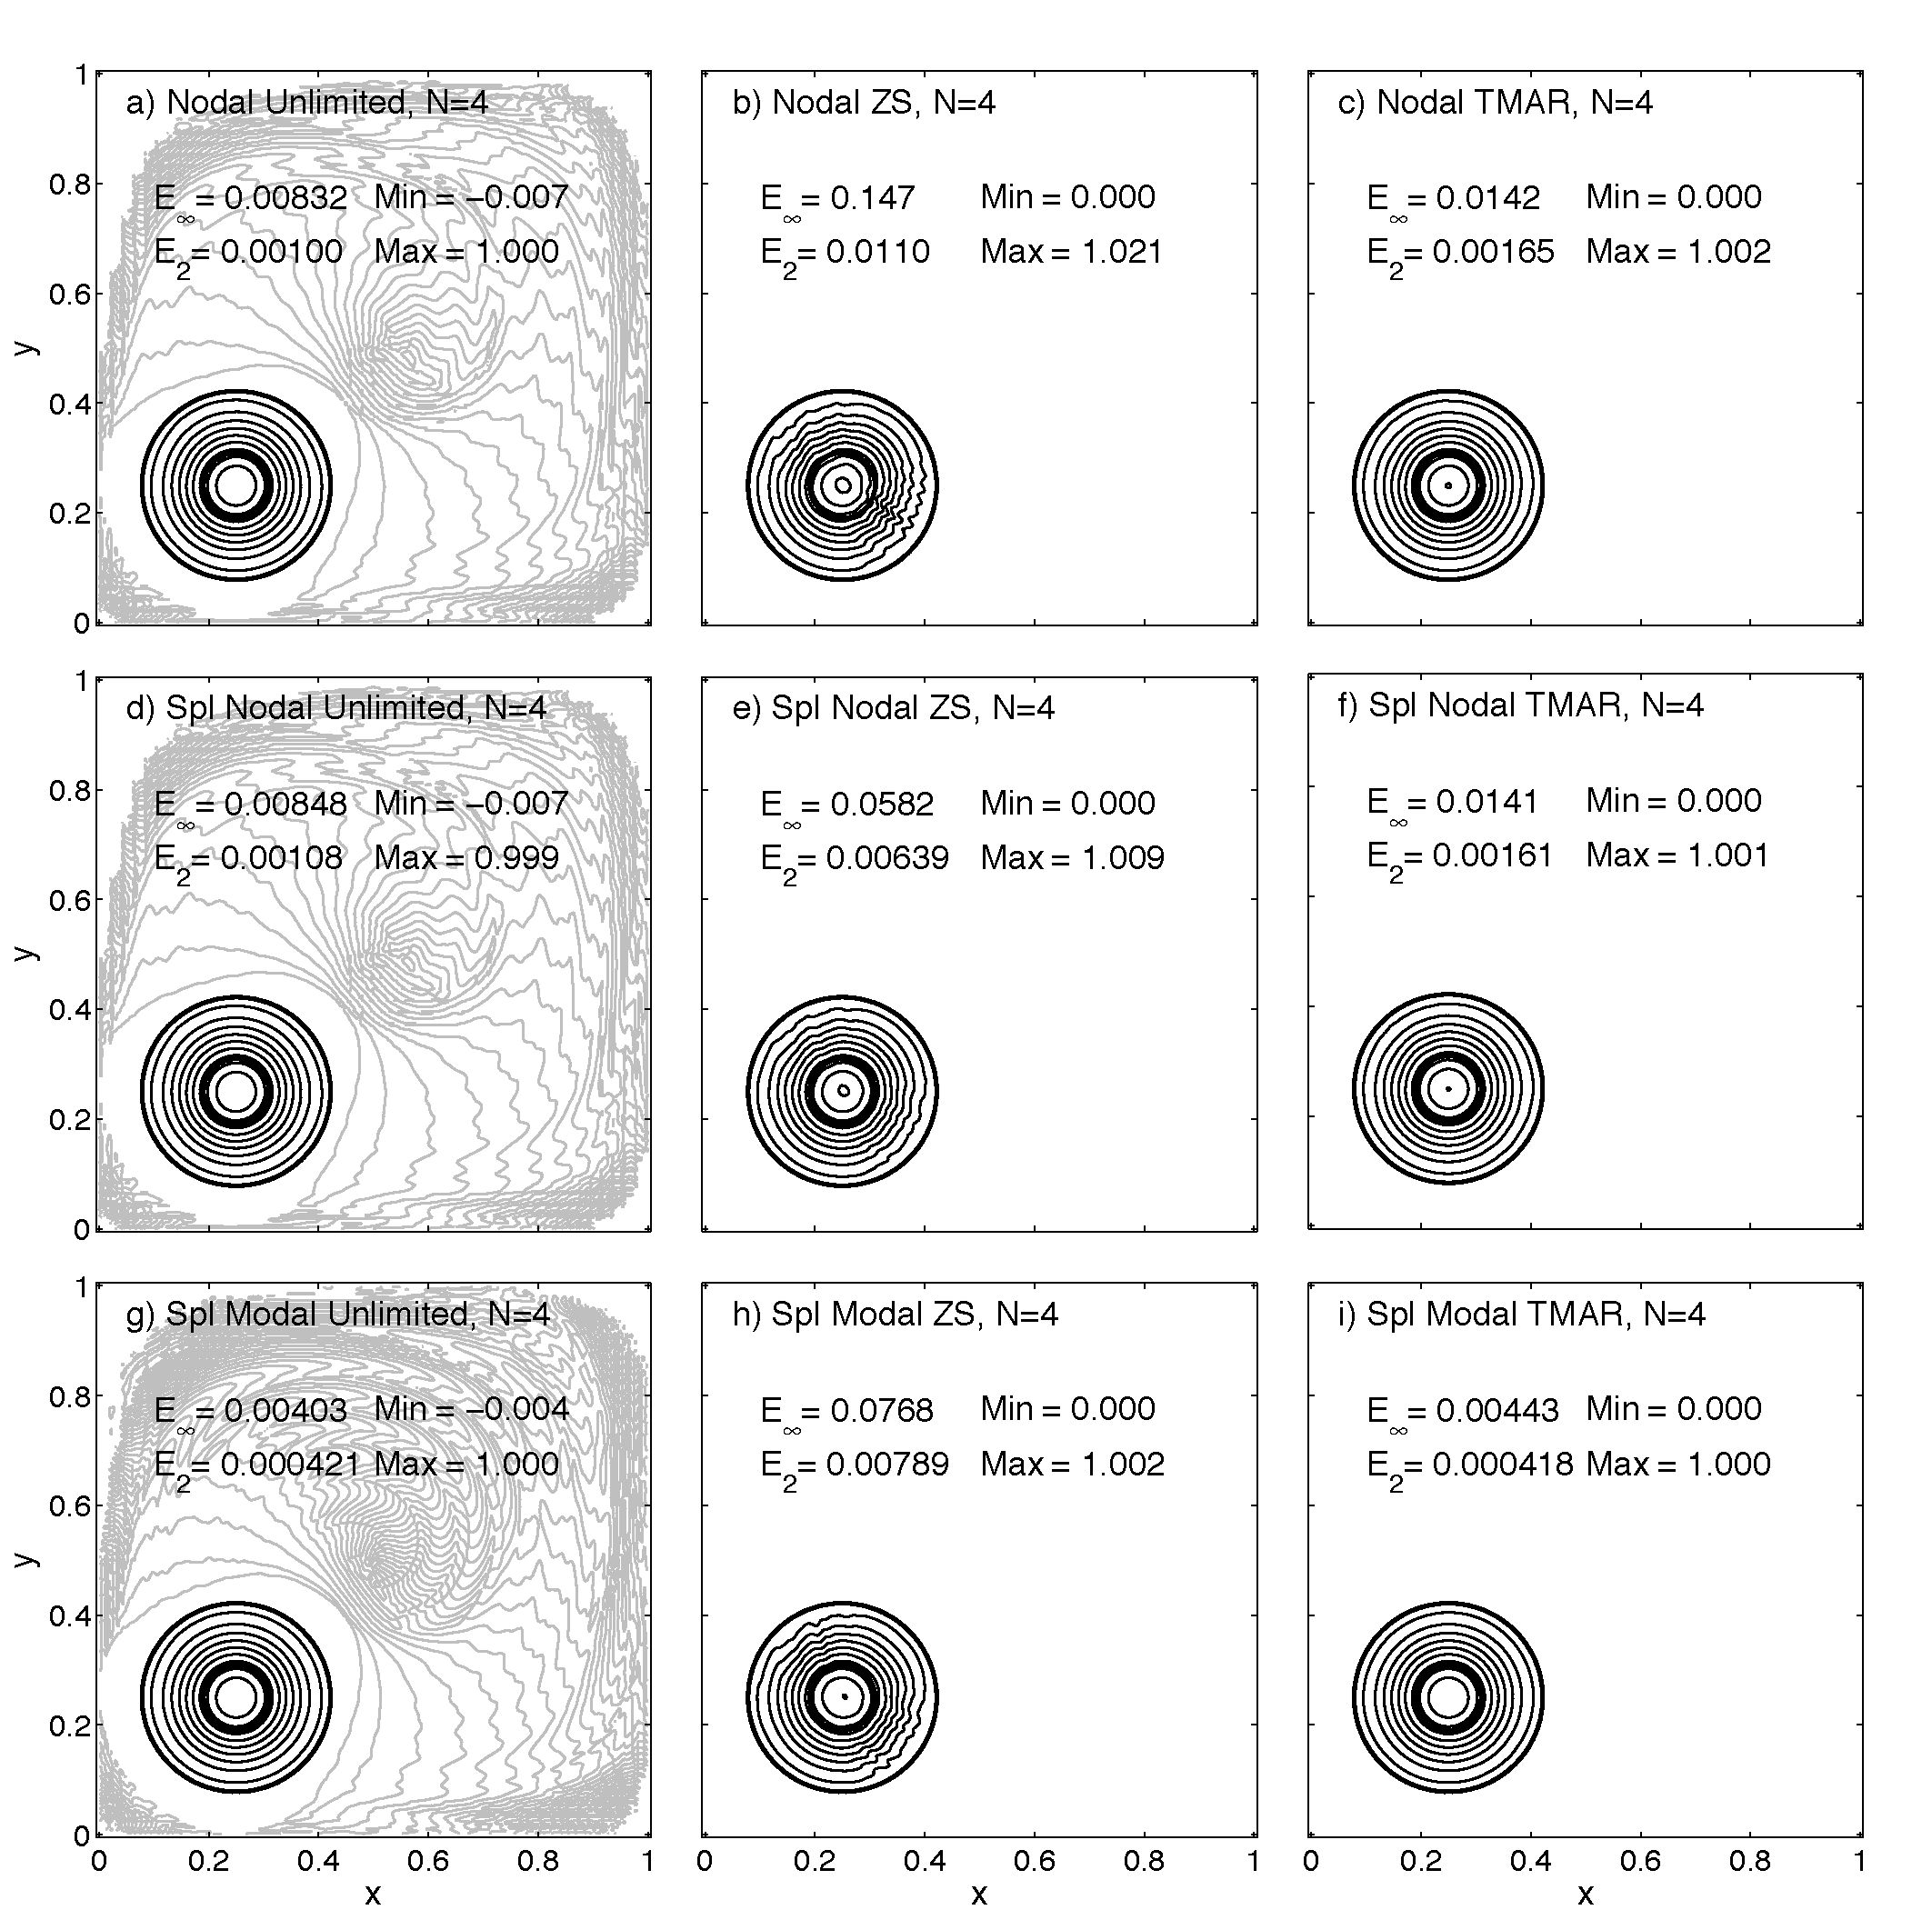
\includegraphics[width=\textwidth]{figs/2d/_defCosbell_9pan_48e.pdf}
\caption{Same as Figure~\ref{fig:2dCosbell24} but using a grid of $48\times48$ elements.}\label{fig:2dCosbell48}
\end{figure}

We also investigate the impact of the limiters on $p$-refinement in two-dimensions. In order to isolate the impact of the limiters as a function of polynomial degree only, Figure~\ref{fig:2dCosbellPref} shows the results of the limited and unlimited unsplit nodal methods for the deformation flow as the polynomial degree is changed while maintaining a constant total degrees of freedom. In each panel there are a total of 120 DOFs along each coordinate. Panels a), b), and c) use a $30 \times 30$ element grid with $N=3$ (4 DOF along each coordinate per element). Panels d), e), and f) increase the local polynomial degree to $N=4$ but simultaneously coarsen the number of elements to a $24 \times 24$ grid. Lastly, panels g), h), and i) use a $20 \times 20$ element grid with $N=5$. The time steps taken for each method are again chosen to remain no greater than 95\% of the maximum value that will maintain non-negativity. The first column of Figure~\ref{fig:2dCosbellPref} illustrates the effects of $p$-refinement on the unlimited method. Despite having an identical number of degrees of freedom, the results obtained using higher degree polynomial reconstructions show a slight improvement in both error norms as well as in the magnitudes of undershoots. The higher degree results also better maintain the circular symmetry and approximate the maximum value of the final solution better than in the cubic case. Similar to the earlier $p$-refinement results shown in Figure~\ref{fig:cosConv-p}, the ZS results in the second column of Figure~\ref{fig:2dCosbellPref} are increasingly degraded as $N$ is increased. This suggests that the ZS limiter will require more degrees of freedom in order to produce a satisfactory result for higher degree polynomial truncations despite the problem remaining unchanged. By comparison, in the last column we see that although the TMAR limiter does have an impact on the error at higher orders, it nevertheless maintains a similar type of improvement that is present in the unlimited solutions as the degree of the local polynomial approximation is increased.

\begin{figure} 
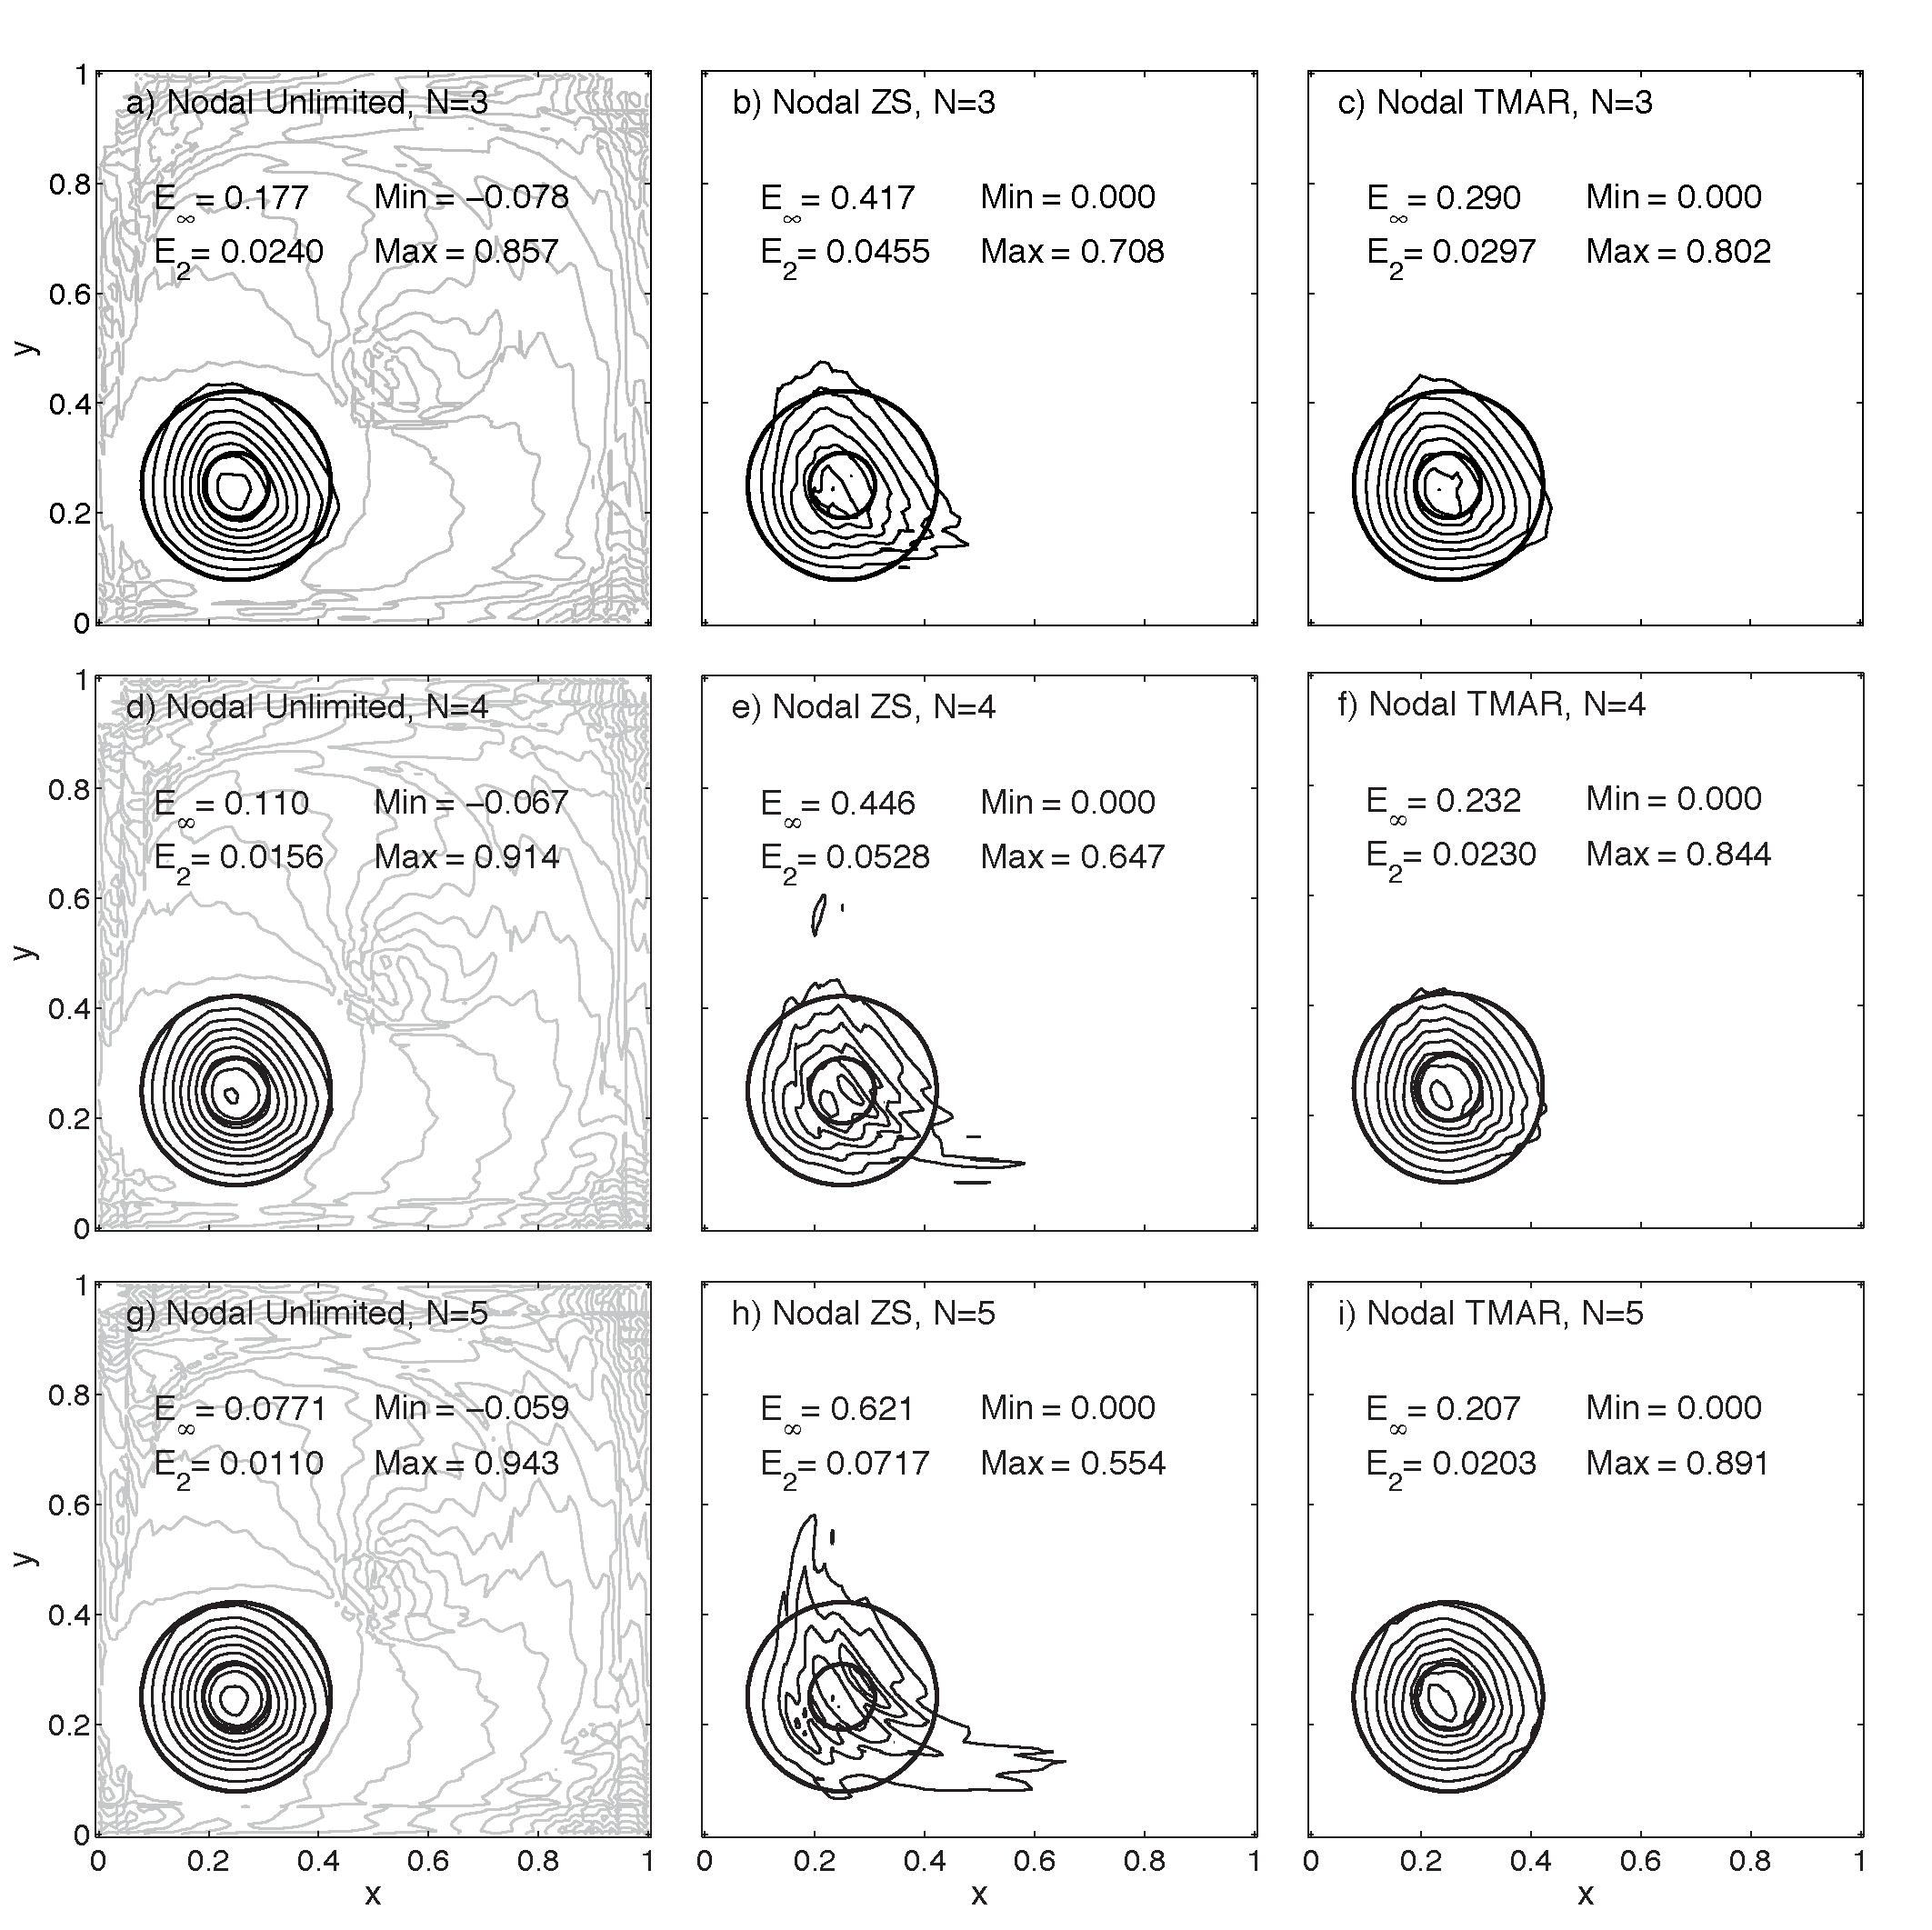
\includegraphics[width=\textwidth]{figs/2d/_defCosbell_9pan_pref.pdf}
\caption{Impact of polynomial refinement on tracer concentration fields at $t=T$. Each panel uses the same 120 total DOFs along each coordinate. Limiting schemes and degree of polynomial truncation are listed in each panel. Contours are every 0.1 and negative contours are highlighted in light gray. Exact solution contours at 0.05 and 0.75 shown in heavy solid lines}\label{fig:2dCosbellPref}
\end{figure}

The difference in performance between the TMAR and ZS limiters for these tests can in part be explained by comparing their impact on individual nodes. While both limiters involve a linear rescaling which is applied to non-negative nodal values, the modifications made to negative nodes are different. As a consequence of the linearity of the ZS limiter, when the local polynomial is modified so that the largest magnitude negative value is scaled to zero, other more minor undershoots are moved into positive values. In contrast, where the TMAR limiter is active, all negative nodal values are truncated to zero which results in a smaller modification for most of the negative nodal values. Furthermore, if an undershoot is at a node which contributes relatively little to the element-averaged density, in the TMAR limiter it has a correspondingly small effect on the magnitude of the rescaling ratio used. On the other hand, any single negative value can solely determine the strength of the rescaling in the ZS limiter. These factors combined allow the TMAR limiter to impose a less substantial damping on the original polynomial. 

\begin{figure} 
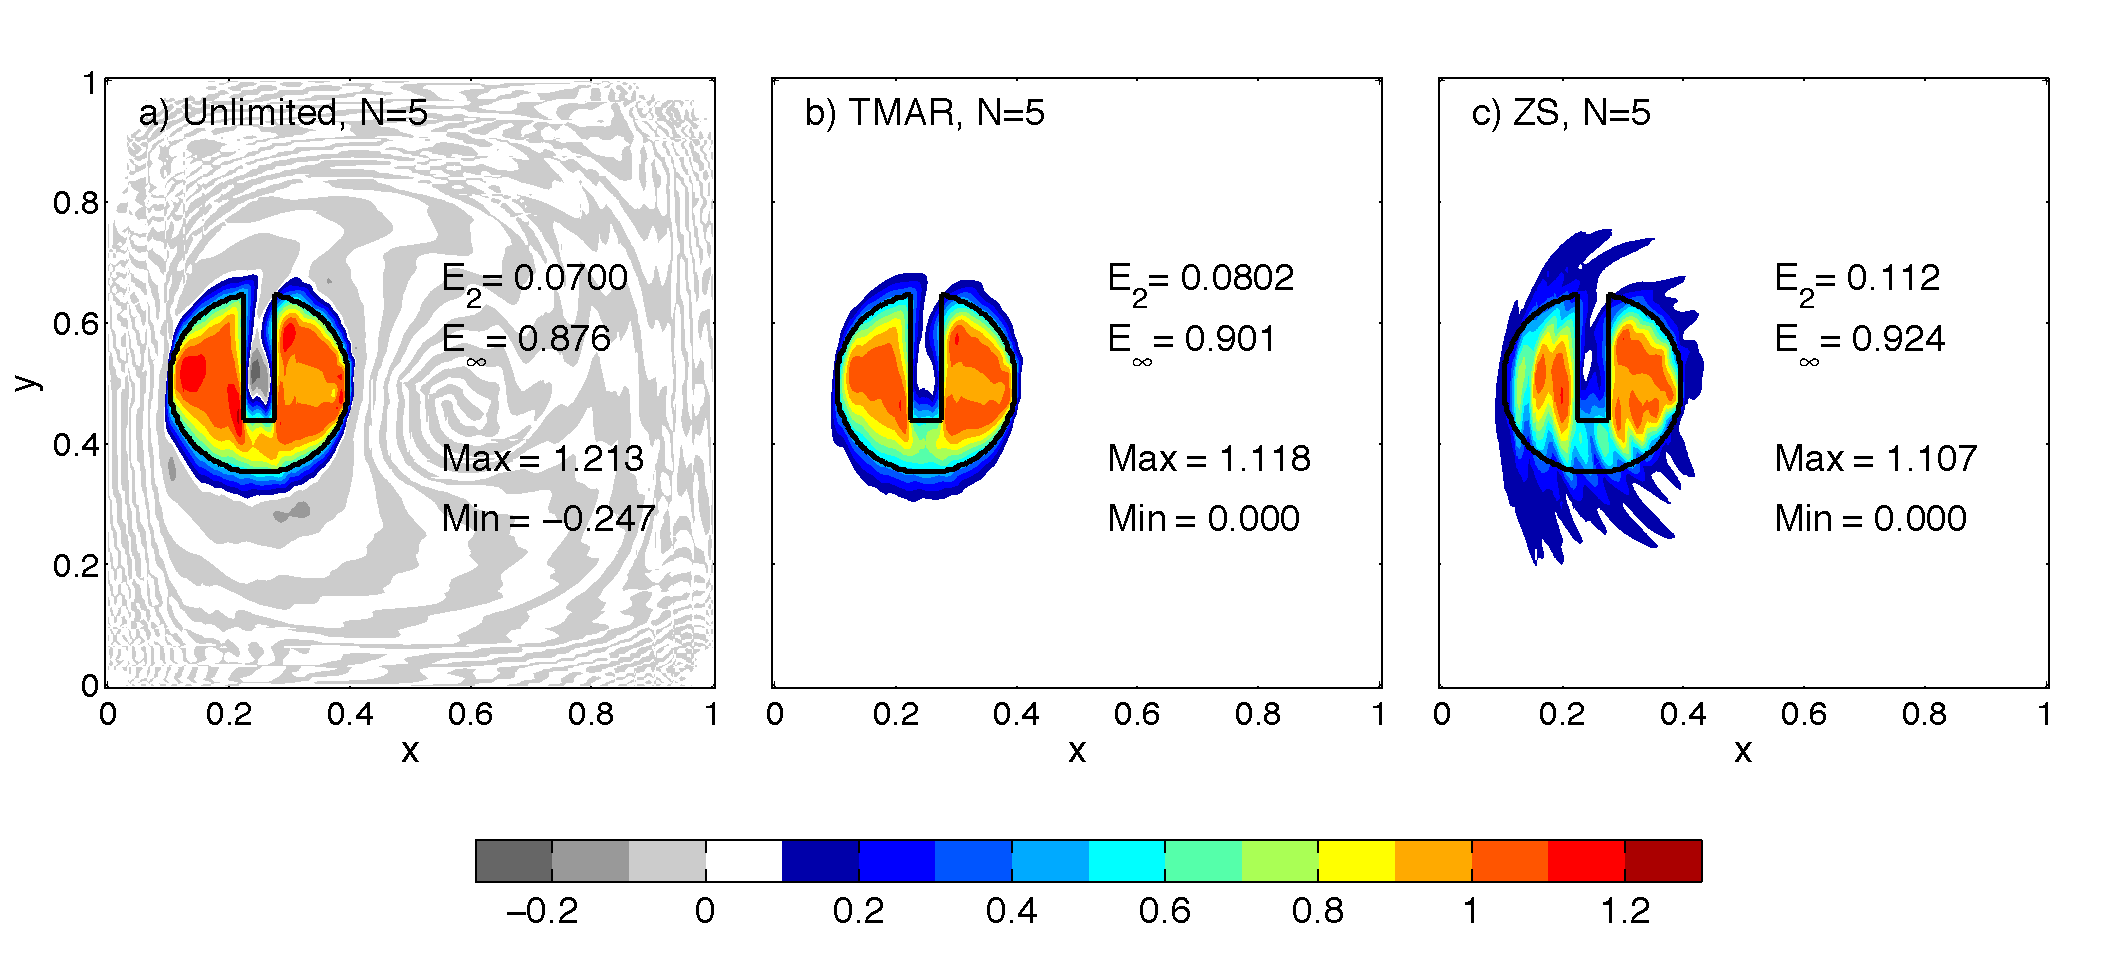
\includegraphics[width=\textwidth]{figs/2d/defCyl_3panel.pdf}
\caption{Tracer concentration field for a slotted cylinder at $t=T$. Contours are every 0.1 and negative regions are highlighted in light gray. Exact solution is outlined by the heavy solid line.}\label{fig:2dCyl}
\end{figure}

Finally, to examine the behavior of these limiters on a 2D flow with actual discontinuities,  the smooth initial tracer field used in the previous tests is replaced by a unit--amplitude slotted cylinder of radius 0.15 centered at $(x_0\, , y_0) = (0.25\,,0.5)$.  The slot, in which the tracer density is zero, includes all points within the cylinder for which $|x-x_0| < 0.025$ and  $y > y_0 + 0.0625$.  Figure \ref{fig:2dCyl} compares the solutions at time $T$ obtained using no limiting, TMAR limiting, and ZS limiting with $N=5$ and $32$ elements (for a total of 192 DOF) along each axis. Due to the discontinuous initial data, the maximum magnitude of overshoots and undershoots in the unlimited solution have increased to about $20\%$ of the initial height of the cylinder and the oscillations away from the cylinder are more pronounced. Even so, the overall structure of the TMAR solution remains similar to the non-negative portion of the unlimited solution. The ZS limiter does remove the negative undershoots, but simultaneously produces short-wavelength noise which distorts the solution. In particular, it erroneously increases the amplitude of the solution within the slotted section of the cylinder which should be vacant.

\section{Computational efficiency} \label{sec:Efficiency}

We now turn to comparing the computational efficiency of the schemes used to obtain the solutions in the preceding two-dimensional deformation tests. The efficiency of a given scheme is a function of the maximum time step allowed by that scheme, the work required per time step, and the accuracy of the result at a given spatial and temporal resolution.  The work per time step is both machine dependent and influenced by the efficiency of the code written for its implementation. All of our results are obtained using the same computing resource, and we have endeavored to impose a similar degree of optimization in the FORTRAN codes used to implement these methods. Despite these efforts, the following results are subject to the caveat that they are still somewhat machine and implementation specific.

Both the ZS and TMAR limiters make a modification to the original DG polynomial in two stages. Since it is possible that each node will have to be adjusted during the second stage of the limiting using both methods, the primary difference in the work per time step is found during the first stage adjustment. In \cite{Zhang:2011aa}, it was noted that a modification to the original algorithm could be made which reduces the number of times the approximating polynomial needs to be evaluated. For a degree $N$ reconstruction, the ZS algorithm uses $L$ points along each boundary where $L$ is the smallest integer such that $2L-3 \geq N$. According to the updated ZS algorithm the approximating polynomial is evaluated at these $L$ points along each boundary plus an additional point within the element. Therefore, the total number of additional polynomial evaluations required is given by $4L+1$. In the worst-case, the two-dimensional FCT step used in the TMAR limiter requires adjusting all of the pointwise fluxes out of the element. Since there are $N+1$ such fluxes along each interface, the FCT step of the TMAR limiter could require as many as $4N+4$ modifications. For both methods the number of adjustments made scales linearly with polynomial degree, however in general the TMAR adjustment will require more modifications to be made. Therefore we expect that the ZS limiter will require less work per time step. The second column in Table~\ref{timingTable} lists the normalized average CPU time spent for a single time step for the ZS and TMAR methods which have been applied to the $C^3$ cosine bell deformation test using $N=4$ and $192\times192$ elements. As the discussion above predicted, the ZS method is faster on average for a single time step than the TMAR limiter and is slightly slower than the unlimited method. 

\begin{table}[!hb]
\begin{tabular}{lcc}
\toprule
  Method & CPU time/step & Total Time \\
\midrule
Unlimited & 1.00 & 1.00  \\
ZS & 1.22 & 3.68  \\
TMAR & 1.34 & 1.34  \\
\bottomrule
\end{tabular}
\caption{Work per time step and total time required to integrate deformation test for ZS and TMAR limiters applied to unsplit DG using $N=4$ and a $192\times192$ element grid. Values normalized by the unlimited method.}
\label{timingTable}
\end{table}

While the previous discussion compares the work required per time step, it does not take into account the differences in permissible time steps between methods. The time step chosen for the ZS scheme must satisfy the more restrictive bound \eqref{eqn:2dZScfl} to guarantee positivity, while the TMAR maintains the same maximum time step chosen for the stability of the unlimited method. To reflect the influence of the maximum time step on computational efficiency, the final column of Table~\ref{timingTable} lists the normalized total integration time for both limiters for the same deformation test. From this, we see that due to the positivity condition \eqref{eqn:2dZScfl}, the ZS method takes more total time to complete its integration despite being more efficient for a single time step.

\begin{figure}[!ht]
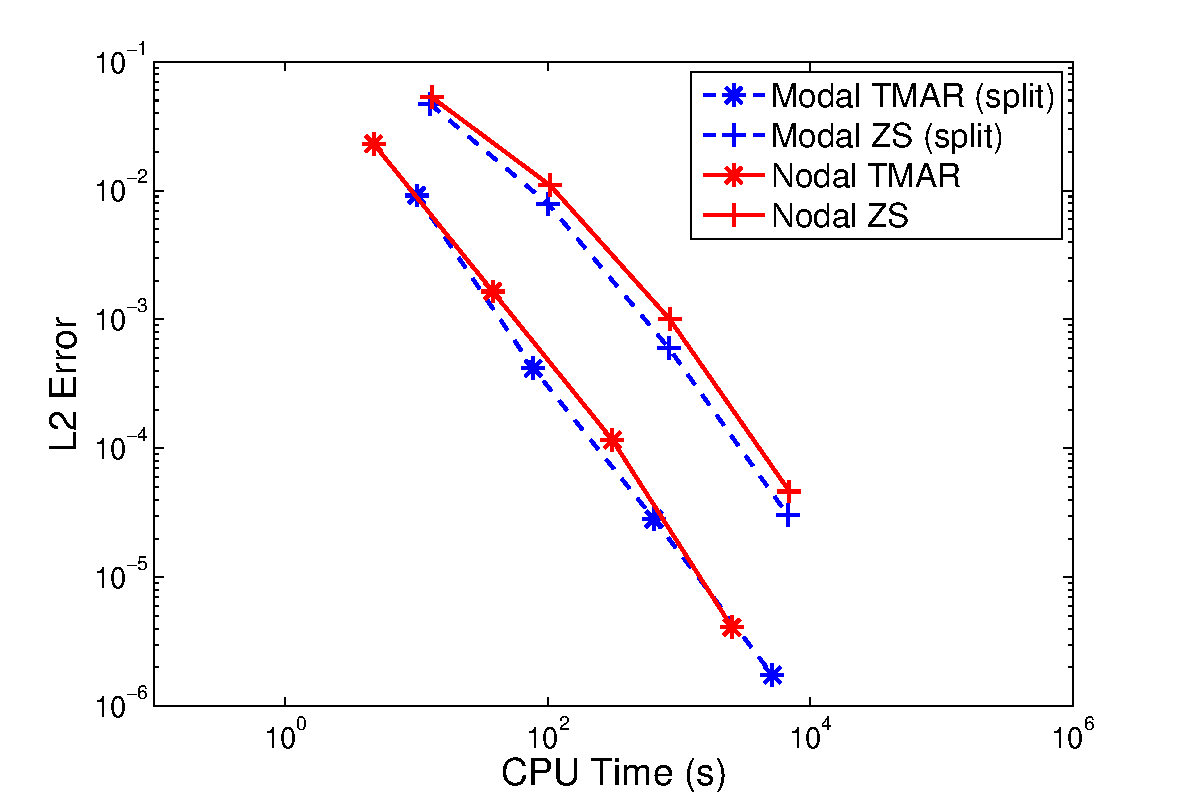
\includegraphics[width=0.74\textwidth]{figs/2d/cosbellDef_L2Cpu.pdf}
\caption{$L_2$ norm of error as a function of computational time spent to integrate the $C^3$ cosine bell deformation with $N=4$. Data points indicate numerical simulations using 24, 48, 96 and 192 elements along each coordinate. }
\label{fig:L2cpu}
\end{figure}

Another key measure of efficiency is the time required to obtain a solution of a desired accuracy. Figure~\ref{fig:L2cpu} plots the CPU time taken for integration versus the $L^2$ error of the resulting approximation for the deformation flow problem using fourth degree polynomials. The data points plotted use 24,48, 96, and 192 elements along each coordinate axis. From this figure we can see that at all resolutions, substantially more accurate results are obtained using the TMAR scheme as the resolution is refined. Additionally, the figure illustrates that the split and unsplit methods produce similarly accurate results for a given length of integration. Most importantly, Figure~\ref{fig:L2cpu} indicates that for a given desired $L^2$ error (of less than $10^{-2}$), a solution can be generated with the least computational effort using the TMAR limiter. 

\section{Conclusion} \label{sec:conc}
In this paper we have introduced a positivity preserving limiter for discontinuous Galerkin approximations to the scalar advection equation. The proposed limiter is appropriate to apply when the analytic solution to the PDE also satisfies a positive definite principle. Our approach truncates the negative nodal values and applies a mass aware rescaling (TMAR) to the remaining positive nodal values. The TMAR scheme can be easily implemented as an alternative to existing limiting techniques with similar computational effort. Like the ZS limiter, this approach preserves the order of accuracy of the unlimited scheme under $h$--refinement. Empirical tests also suggest that the TMAR limiter performs nearly as well as the unlimited scheme under $p$--refinement. In contrast to the ZS limiter, the TMAR limiter does not rescale any negatives into positive values. The advantages of the TMAR limiting are most apparent when using a high degree polynomial truncation because spurious negative nodal values near element boundaries which contribute little to the total element mass also exert only a minor influence on the TMAR rescaling.

%%%%%%%%%%%%%%%%%%%%%%%%%%%%%%%%%%%%%%%%%%%%%%%%%%%%%%%%%%%%%%%%%%%%%
% ACKNOWLEDGMENTS
%%%%%%%%%%%%%%%%%%%%%%%%%%%%%%%%%%%%%%%%%%%%%%%%%%%%%%%%%%%%%%%%%%%%%
%
\acknowledgments
Start acknowledgments here.

%%%%%%%%%%%%%%%%%%%%%%%%%%%%%%%%%%%%%%%%%%%%%%%%%%%%%%%%%%%%%%%%%%%%%
% APPENDIXES
%%%%%%%%%%%%%%%%%%%%%%%%%%%%%%%%%%%%%%%%%%%%%%%%%%%%%%%%%%%%%%%%%%%%%
%
% Use \appendix if there is only one appendix.
%\appendix

% Use \appendix[A], \appendix}[B], if you have multiple appendixes.
%\appendix[A]

%% Appendix title is necessary! For appendix title:
%\appendixtitle{}

%%% Appendix section numbering (note, skip \section and begin with \subsection)
% \subsection{First primary heading}

% \subsubsection{First secondary heading}

% \paragraph{First tertiary heading}

%% Important!
%\appendcaption{<appendix letter and number>}{<caption>} 
%must be used for figures and tables in appendixes, e.g.,
%
%\begin{figure}
%\noindent\includegraphics[width=19pc,angle=0]{figure01.pdf}\\
%\appendcaption{A1}{Caption here.}
%\end{figure}
%
% All appendix figures/tables should be placed in order AFTER the main figures/tables, i.e., tables, appendix tables, figures, appendix figures.
%
%%%%%%%%%%%%%%%%%%%%%%%%%%%%%%%%%%%%%%%%%%%%%%%%%%%%%%%%%%%%%%%%%%%%%
% REFERENCES
%%%%%%%%%%%%%%%%%%%%%%%%%%%%%%%%%%%%%%%%%%%%%%%%%%%%%%%%%%%%%%%%%%%%%
% Make your BibTeX bibliography by using these commands:
 \bibliographystyle{ametsoc2014}
 \bibliography{references}


%%%%%%%%%%%%%%%%%%%%%%%%%%%%%%%%%%%%%%%%%%%%%%%%%%%%%%%%%%%%%%%%%%%%%
% TABLES
%%%%%%%%%%%%%%%%%%%%%%%%%%%%%%%%%%%%%%%%%%%%%%%%%%%%%%%%%%%%%%%%%%%%%
%% Enter tables at the end of the document, before figures.
%%
%
%\begin{table}[t]
%\caption{This is a sample table caption and table layout.  Enter as many tables as
%  necessary at the end of your manuscript. Table from Lorenz (1963).}\label{t1}
%\begin{center}
%\begin{tabular}{ccccrrcrc}
%\hline\hline
%$N$ & $X$ & $Y$ & $Z$\\
%\hline
% 0000 & 0000 & 0010 & 0000 \\
% 0005 & 0004 & 0012 & 0000 \\
% 0010 & 0009 & 0020 & 0000 \\
% 0015 & 0016 & 0036 & 0002 \\
% 0020 & 0030 & 0066 & 0007 \\
% 0025 & 0054 & 0115 & 0024 \\
%\hline
%\end{tabular}
%\end{center}
%\end{table}

%%%%%%%%%%%%%%%%%%%%%%%%%%%%%%%%%%%%%%%%%%%%%%%%%%%%%%%%%%%%%%%%%%%%%
% FIGURES
%%%%%%%%%%%%%%%%%%%%%%%%%%%%%%%%%%%%%%%%%%%%%%%%%%%%%%%%%%%%%%%%%%%%%
%% Enter figures at the end of the document, after tables.
%%
%
%\begin{figure}[t]
%  \noindent\includegraphics[width=19pc,angle=0]{figure01.pdf}\\
%  \caption{Enter the caption for your figure here.  Repeat as
%  necessary for each of your figures. Figure from \protect\cite{Knutti2008}.}\label{f1}
%\end{figure}

\end{document}